\clearpage
\newpage
\chapter{Background Estimation}
\label{sec:backgroundEstimation}
An essential part of the analysis is the data driven estimation of the QCD background.  
The background estimate relies on extracting the average b-tagging rate of a QCD jet in our signal region.  
We extract this rate by making use of the following sideband.
\section{Substructure Sideband}
\label{sec:sideband}
We define the substructure sideband as events passing all signal region cuts but explicitly 
failing the top jet substructure cut on the number of subjets.  Additionally, to ensure similar parton flavor distributions in the signal region and sideband (Figure \ref{figs:partonflav}), 
we also include subjet CSV discrimination. The top jet sideband is defined as:
\begin{eqnarray}
	140  <  m_{\text{jet}}  <  250 \GeV \\
	N_{\text{subjets}}  \leq  2 \\
	SJ_{\text{CSVMAX}} \geq 0.679 
\end{eqnarray}
The Minimum Pairwise Mass variable described in Section \ref{sec:toptagging} is not defined in this choice of sideband.

\section{QCD Background Estimation}
\label{sec:qcdBackgroundEstimationProcedure}
\label{sec:tagrateparameterization}
The estimation of QCD background is performed by extracting the probability to tag a b jet in the sideband. 
The primary assumption used in background estimation is that the average b-tagging probability 
for QCD multijets in the signal region is nearly identical to the sideband. Figure \ref{figs:partonflav}  shows the parton flavor distribution for signal region and sideband in QCD MC, the
 nearly identical composition can be considered motivation for the previous assumption.

To extract a QCD background estimate, we weight the events that pass the full selection in the signal region before the b-tagging requirement is applied by 
the average b-tagging probability (measured in the top jet sideband).  This gives us an accurate expectation of the QCD background in the signal region.
The b-tagging rate is defined as the inverse ratio of the number of b candidate jets, 
defined as $\pt > 370~\GeV$ jets in the hemisphere opposite the top jet to the number of b candidate jets that are b-tagged.  
%This ratio is shown if Figure \ref{figs:partonflav} in bins of parton flavor for signal region and sideband as extracted from QCD Monte Carlo.    

\begin{figure}[htbp]
\begin{center}
\subfigure{\label{figs:partonflavCOMP}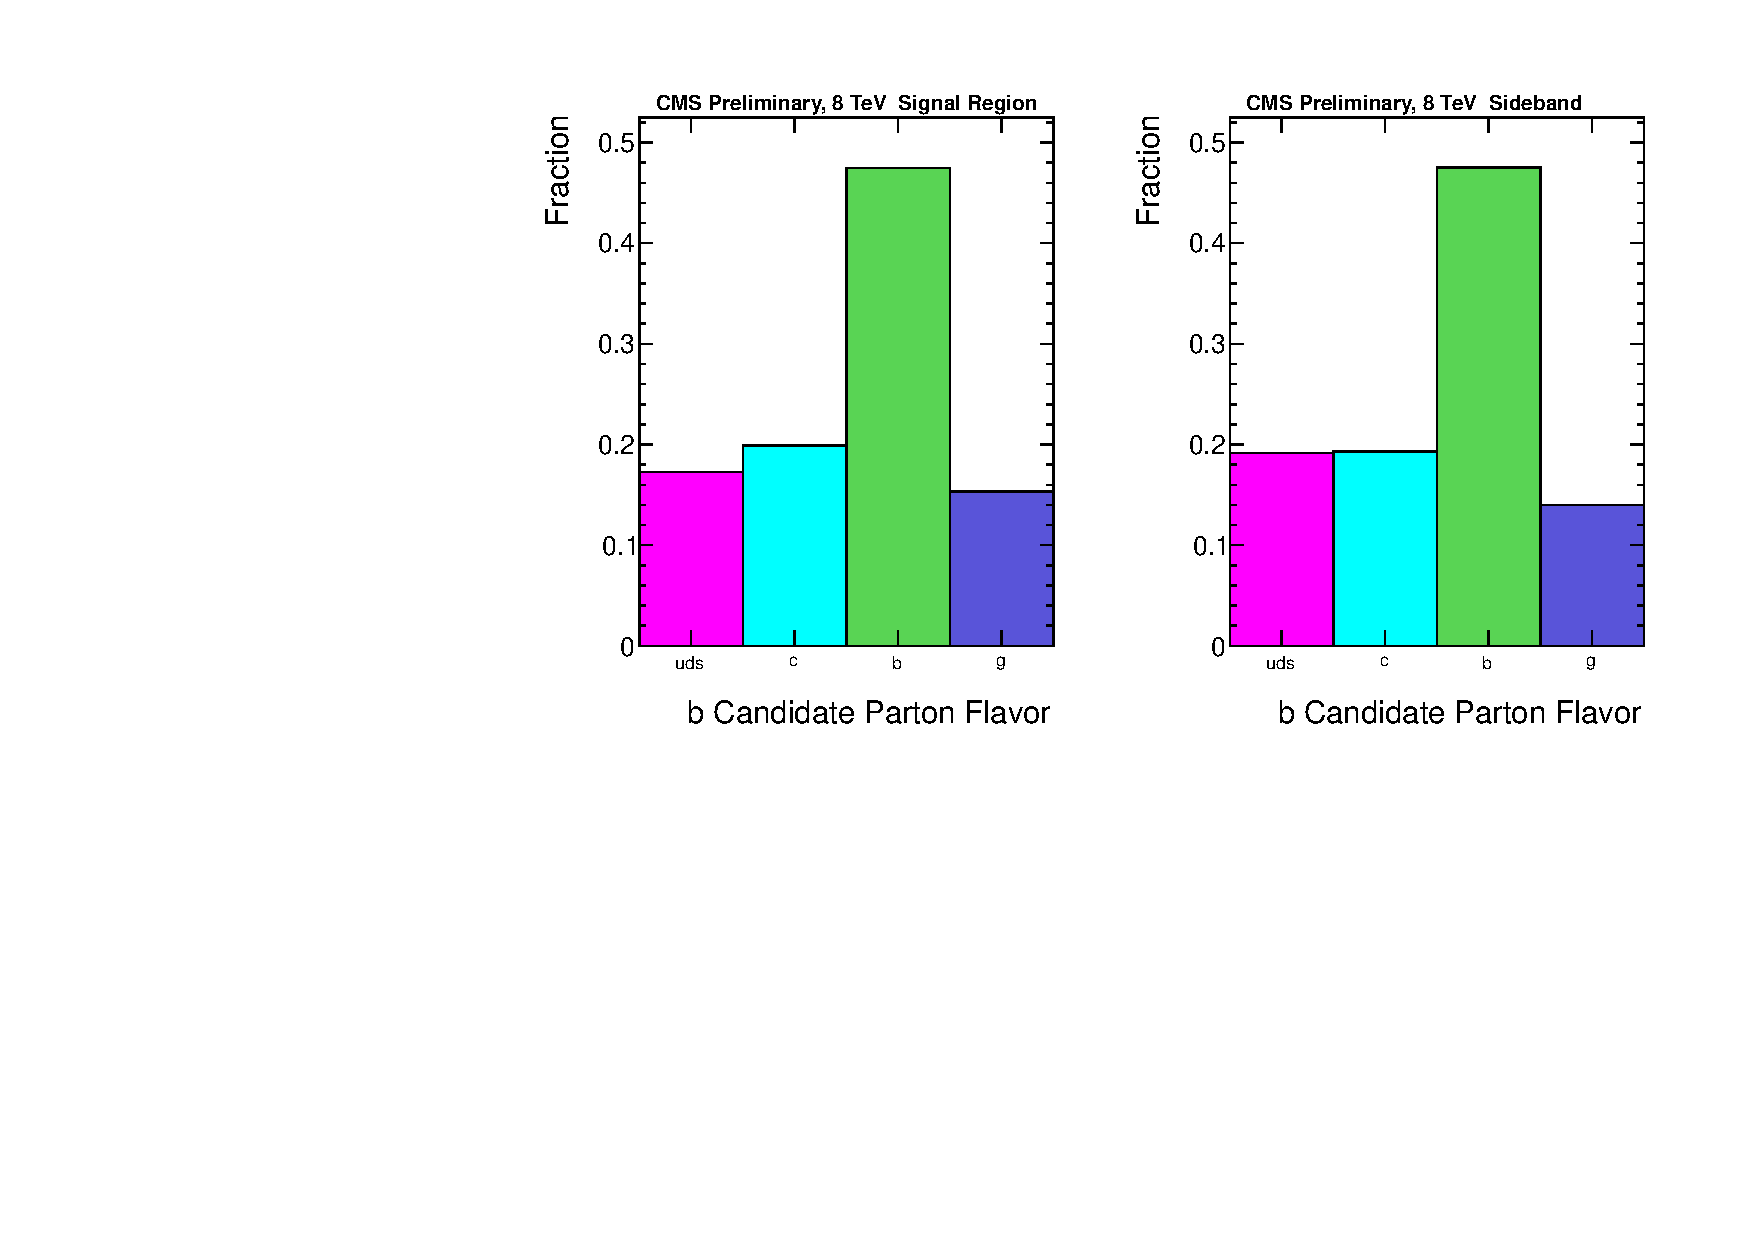
\includegraphics[width=1.0\textwidth]{AN-13-004/figs/partonflavCOMP}}\\ 
\caption{
Comparison of jet parton flavor composition from the signal region and sideband.
%(b) Comparison of average b-tagging rate as a function of jet parton flavor from the signal region and sideband.  
}
\label{figs:partonflav}
\end{center}
\end{figure}

The parameterization of the average b-tagging rate is two dimensional and considers both the $|\eta|$ and $\pt$ of the b candidate jets.  
We break down data into three distinct regions in $|\eta|$. 


\begin{itemize}
	\item \text{Low } $(0.0 < |\eta| \leq 0.5)$
	\item \text{Transition } $(0.5 < |\eta| \leq 1.15)$ 
	\item \text{High } $(1.15 < |\eta| \leq 2.4)$ 
\end{itemize}

The regions in $|\eta|$ are then individually parameterized in $\pt$ to produce the average b-tagging rate.  We perform this parameterization 
of the b-tagging rate in an attempt to constrain the kinematic correlations inherent in b-tagging.

To smooth out the binning of the average b-tagging rate, a study of functional fits was conducted for the average b-tagging rate (see Figure \ref{figs:BKGFITCOMP}).
We chose the bifurcated polynomial fit based on observed representation of the data.  The fitting function is as follows

\begin{eqnarray}
f(x) =
\begin{cases}
p_0+p_1x+p_2(x-\text{a})^2, & \text{if x} < \text{a} \\
p_0+p_1x+p_3(x-\text{a})^2, & \text{if x}\geq\text{a}
\end{cases}
\end{eqnarray}

Here, the parameters $p_0$ through $p_3$ are inputs to the fitting algorithm, and x is the $\pt$ of the b candidate jet.  The parameter a is the bifurcation point, and is chosen manually for each region in $\eta$.
It is chosen to be 500$~\GeV$, 500$~\GeV$, and 550$~\GeV$ for the low, transition, and high $\eta$ regions respectively.
This piecewise function allows for two characteristic ranges to fit a polynomial, which makes a good fit for the different functional forms of the average b-tagging rate regions that we use.

The errors on the average b-tagging rate are then extracted using the full covariance matrix as obtained from output of the fitting 
algorithm.   
Additionally, we assign a systematic uncertainty to cover the choice of the fit function (see Chapter \ref{sec:systematics}) based on several alternative functional forms.
Figure \ref{figs:tagsandprobes8TeV} shows the tags (numerator) and probes (denominator) of the tagging rate.
Figure \ref{figs:tagrateetafit} shows the three fitted average b-tagging rates parameterized in $\pt$.  

%\section{Treatment of QCD Background Events with Double Top Tags}
%\label{sec:dubtags}
%As mentioned in Section \ref{sec:analysisStrategy}, the analysis uses  hemispherically separated dijets as top and b candidates.  
%Because it is not obvious which candidate will be the leading jet, both are considered.  If the event registers a count in either of these configurations, the other is not considered to prevent double counting.  
%However, the QCD background estimate is based on the probability of recording a count and thus the cut to prevent double counting should not be applied when filling the QCD background.  
%This type of event occurs when both the leading and sub leading jet are top tagged, and both jets are considered for b-tagging.  
%Note that this does not impact the treatment of ttbar, and these events are simply of rare QCD origin (see Section \ref{sec:ttSubtraction}). 
%An event that records two counts in the background estimation has the physical meaning that the event has two chances to tag a b jet.

\section{$\ttbar$ Subtraction}
\label{sec:ttSubtraction}
\label{sec:bsttSubtraction}
The $\ttbar$ contribution to background is computed from Monte Carlo that passes the full selection. To avoid double-counting, we must remove $\ttbar$ from our QCD estimate. 
In creating the b-tagging rate, the $\ttbar$ contribution to the numerator and denominator is subtracted away using $\ttbar$ Monte Carlo. 
Additionally, we account for the $\ttbar$ contamination of the QCD background estimate by applying 
the average b-tagging rate to $\ttbar$ Monte Carlo in the same way as data.  This is a measure of $\ttbar$ that is expected to fall 
through the QCD background estimate and is subtracted away. 

%We can similarly consider the possible effect of the single-top contribution to this tag rate. 
%However, due to the very low background from single-top, we find that we do not need to modify the average b-tagging rate. 
%Table \ref{table:singletop} shows a comparison of the various contribution to the average b-tagging rate.  
%Theoretically, the signal could also be present in the 
%pre tagged and post tagged sample, which could bias the background estimation.  However, in practice it is seen that this effect is a fraction of a 
%percent and is thus much smaller than the uncertainty placed on the background estimation.

\begin{table}
\begin{center}
\begin{tabular}{|c||c|c|c|} 
\hline
  & $\eta_1$ & $\eta_2$ & $\eta_3$ \\
\hline
\hline
pretag QCD & 15922 ($99.77\%$) & 14396 ($99.79\%$) & 5494 ($99.81\%$)\\
tagged QCD & 924 ($99.17\%$) & 847 ($99.16\%$) & 285 ($99.54\%$)\\
pretag $\ttbar$ & 37 ($0.23\%$) & 31 ($0.21\%$) & 11 ($0.19\%$)\\
tagged $\ttbar$ & 8 ($0.83\%$) & 7 ($0.84\%$) & 1 ($0.46\%$)\\
pretag signal at 1300$\GeV$ & 108 ($0.67\%$) & 77 ($0.53\%$) & 17 ($0.30\%$)\\
tagged signal at 1300$\GeV$ & 37 ($3.94\%$) & 24 ($2.87\%$) & 4 ($1.44\%$)\\
pretag signal at 1500$\GeV$ & 62 ($0.39\%$) & 39 ($0.27\%$) & 8 ($0.14\%$)\\
tagged signal at 1500$\GeV$ & 17 ($1.86\%$) & 11 ($1.28\%$) & 2 ($0.67\%$)\\
pretag signal at 1700$\GeV$ & 31 ($0.19\%$) & 19 ($0.13\%$) & 3 ($0.06\%$)\\
tagged signal at 1700$\GeV$ & 8 ($0.82\%$) & 4 ($0.53\%$) & 1 ($0.25\%$)\\
pretag signal at 1900$\GeV$ & 15 ($0.09\%$) & 9 ($0.06\%$) & 1 ($0.02\%$)\\
tagged signal at 1900$\GeV$ & 3 ($0.31\%$) & 2 ($0.20\%$) & 0 ($0.07\%$)\\
pretag signal at 2100$\GeV$ & 7 ($0.04\%$) & 4 ($0.03\%$) & 0 ($0.01\%$)\\
tagged signal at 2100$\GeV$ & 1 ($0.13\%$) & 1 ($0.09\%$) & 0 ($0.03\%$)\\
\hline
\end{tabular}
\end{center}
\caption{Number of tagged and pretagged events for each background sample and percent contribution to overall average b-tagging rates.  Additionally, signal samples are investigated.  
The percents indicated are out of the total QCD + $\ttbar$ expectation and the signal samples are scaled to theory cross-section.}
\label{table:singletop}
\end{table}

\begin{figure}[htcb]
\centering
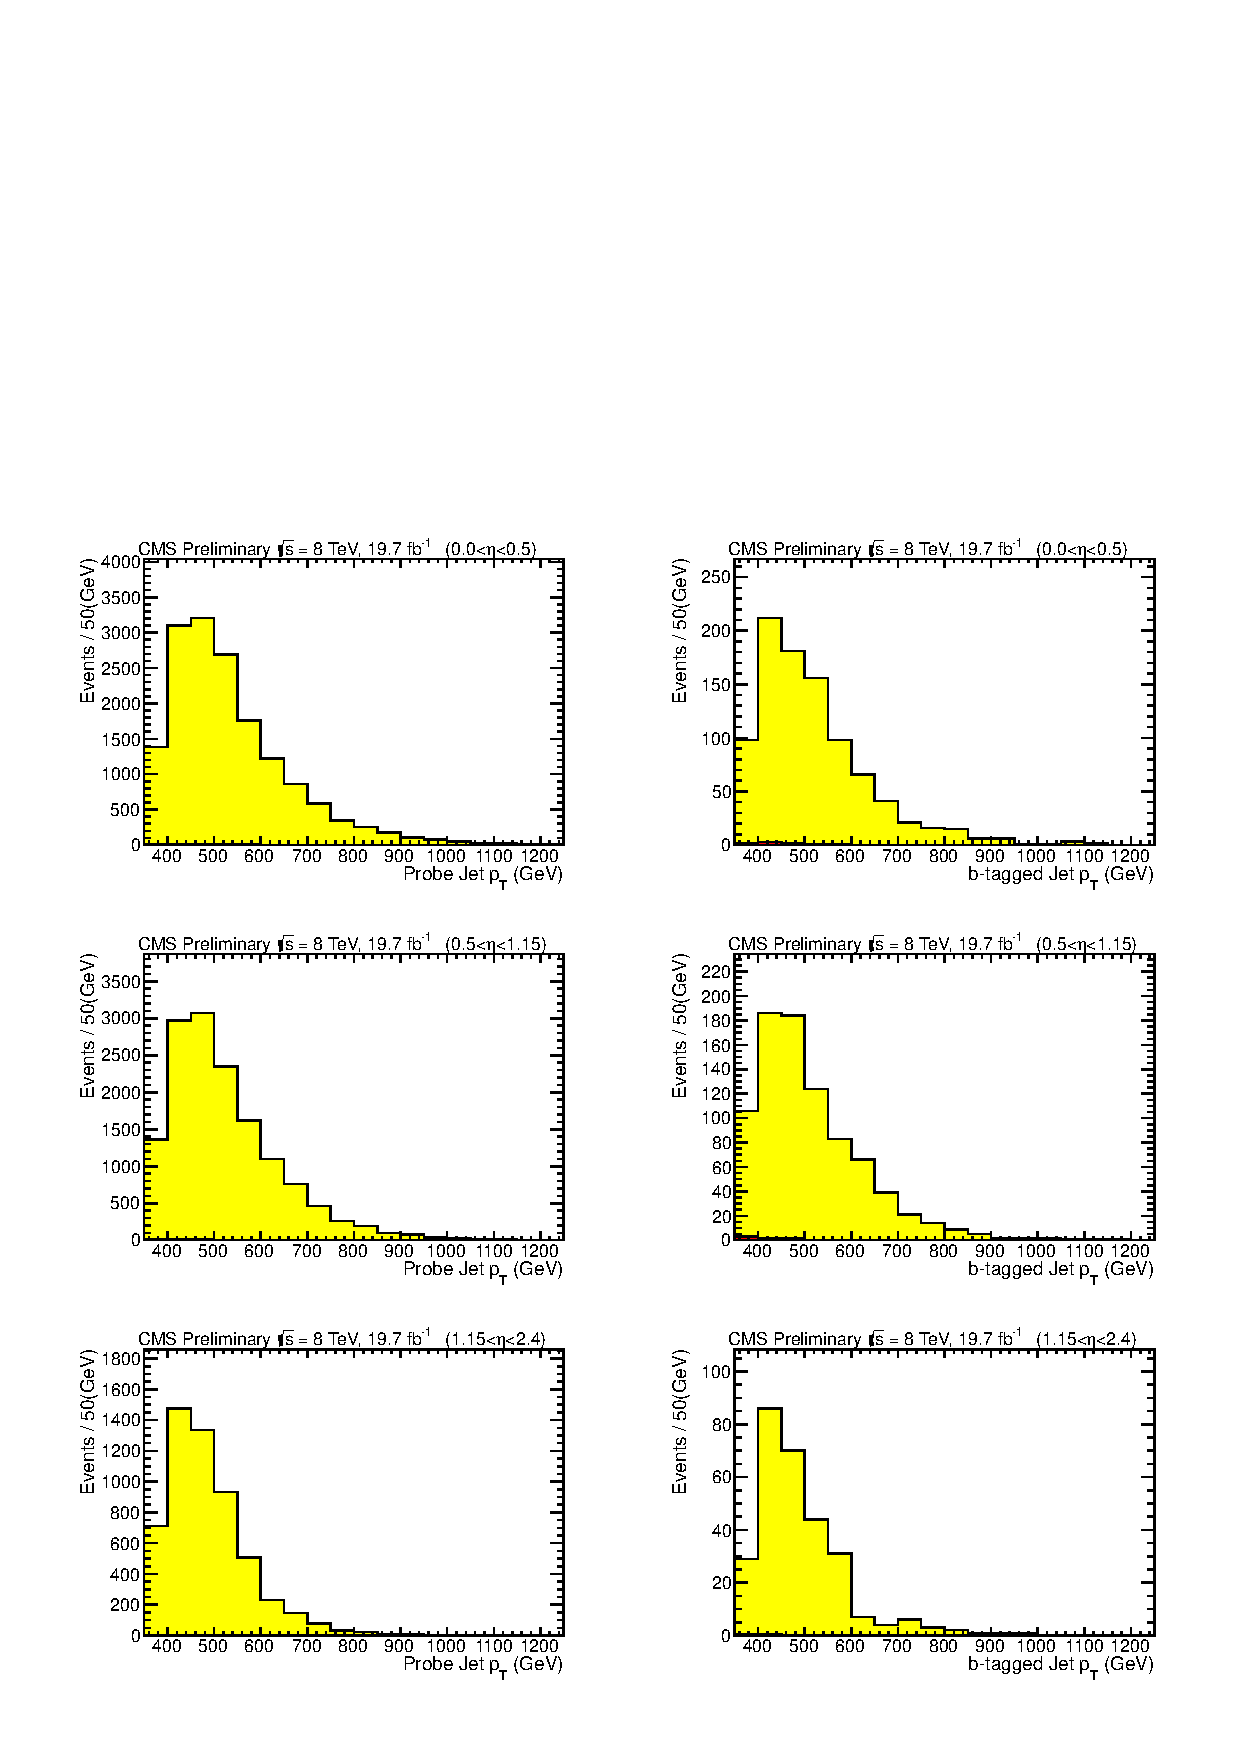
\includegraphics[width=1.0\textwidth]{AN-13-004/figs/tagsandprobes}
\caption{The tags and probes used for the average b-tagging rate in each of the three regions in $|\eta|$ .  Here, tags are the numerator and probes are the denominator of the average b-tagging rate}
\label{figs:tagsandprobes8TeV}
\end{figure}

\begin{figure}[htcb]
\begin{center}
\subfigure{\label{figs:tagrateeta1fit}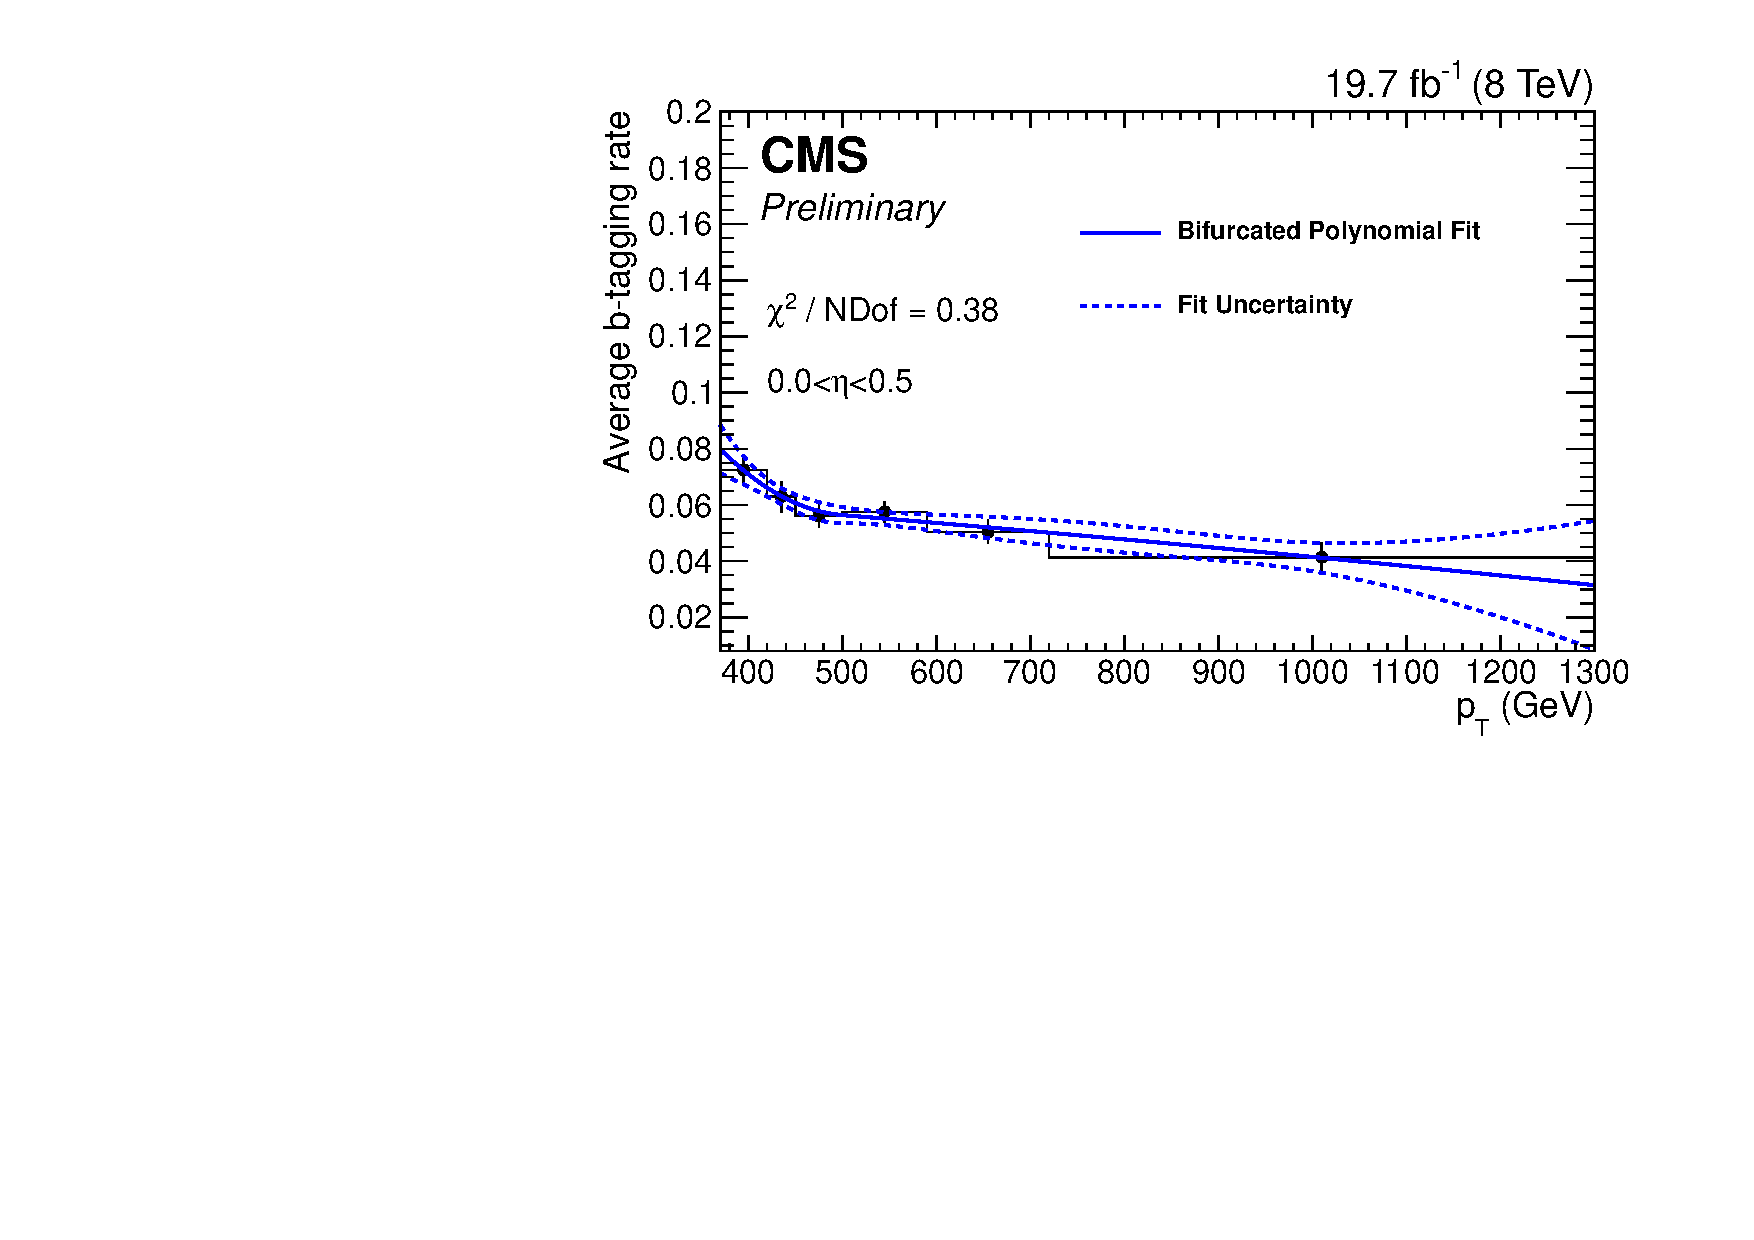
\includegraphics[width=0.7\textwidth]{AN-13-004/figs/tagrateeta1fitBP.pdf}}\\
\subfigure{\label{figs:tagrateeta2fit}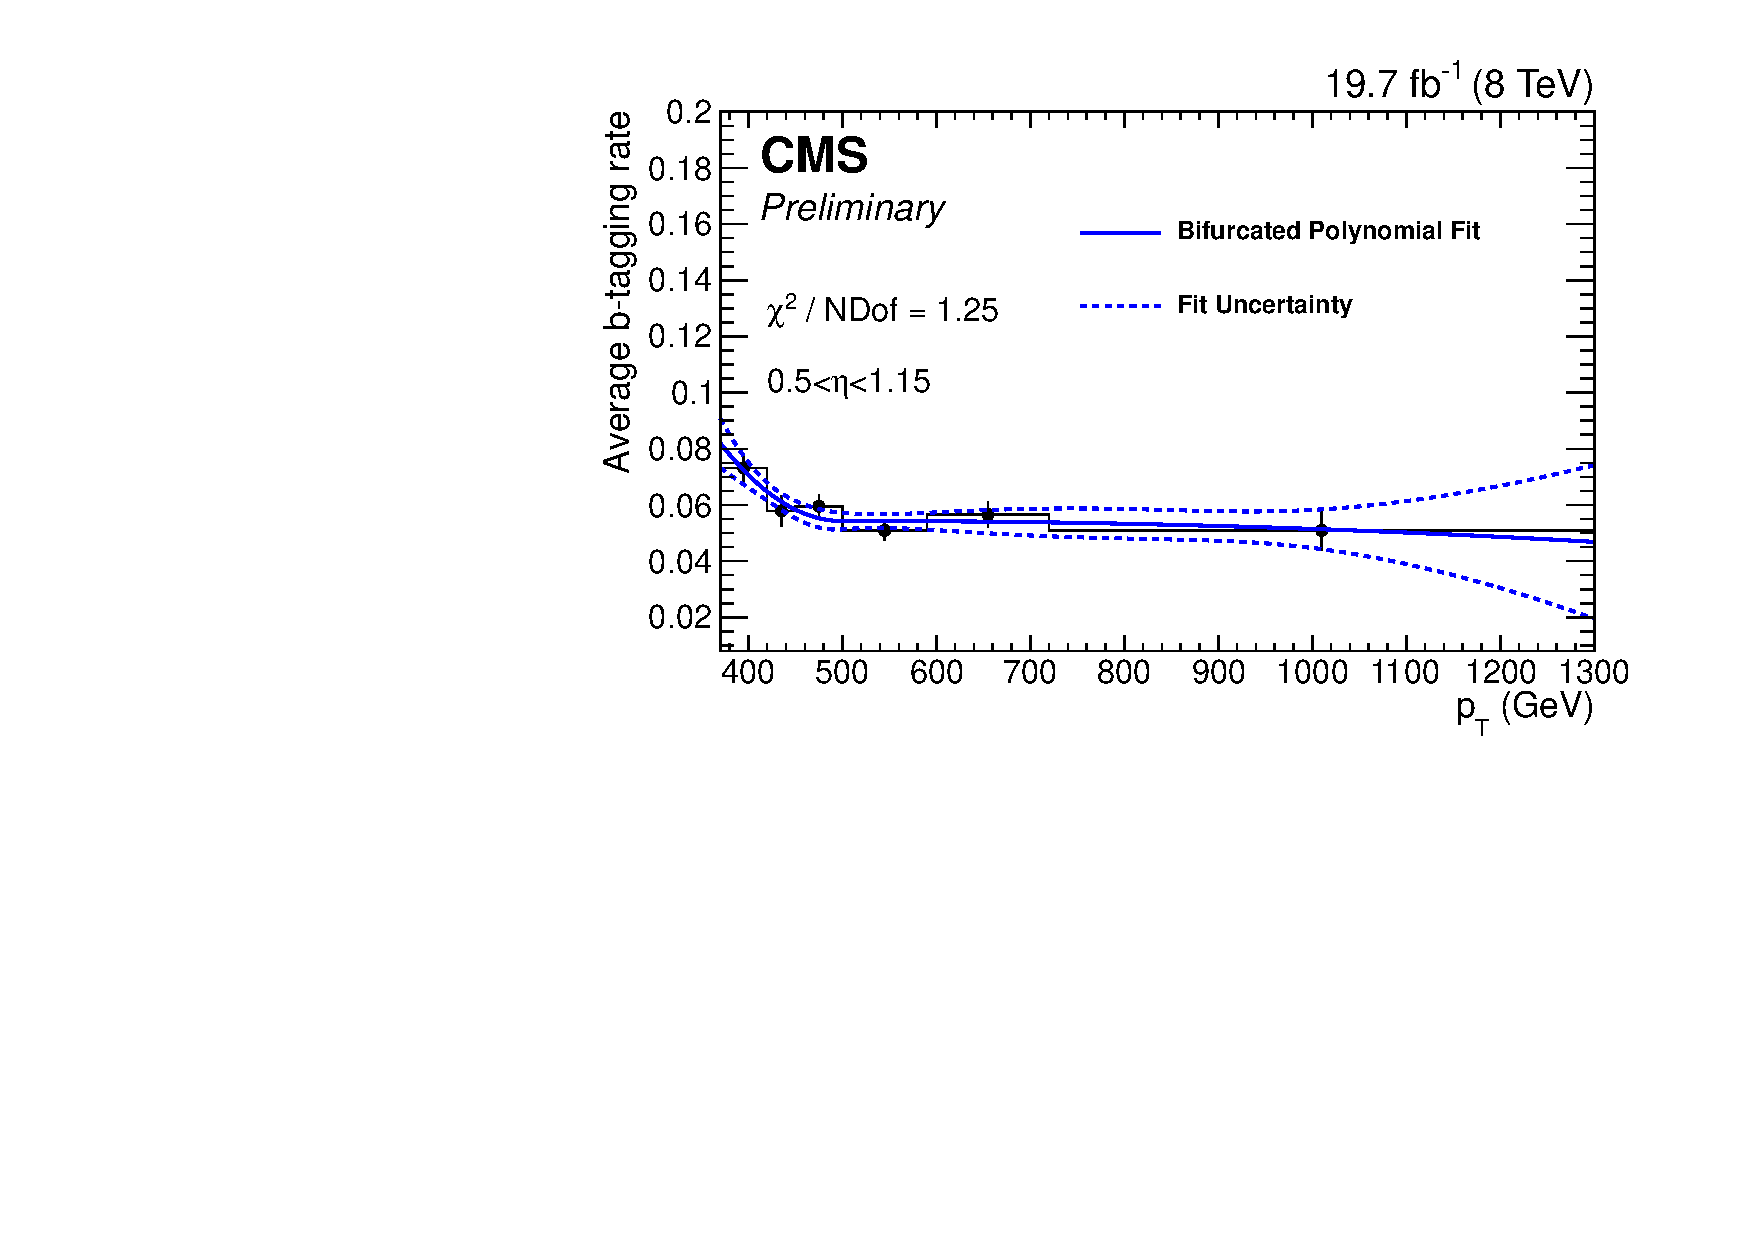
\includegraphics[width=0.7\textwidth]{AN-13-004/figs/tagrateeta2fitBP.pdf}}\\
\subfigure{\label{figs:tagrateeta3fit}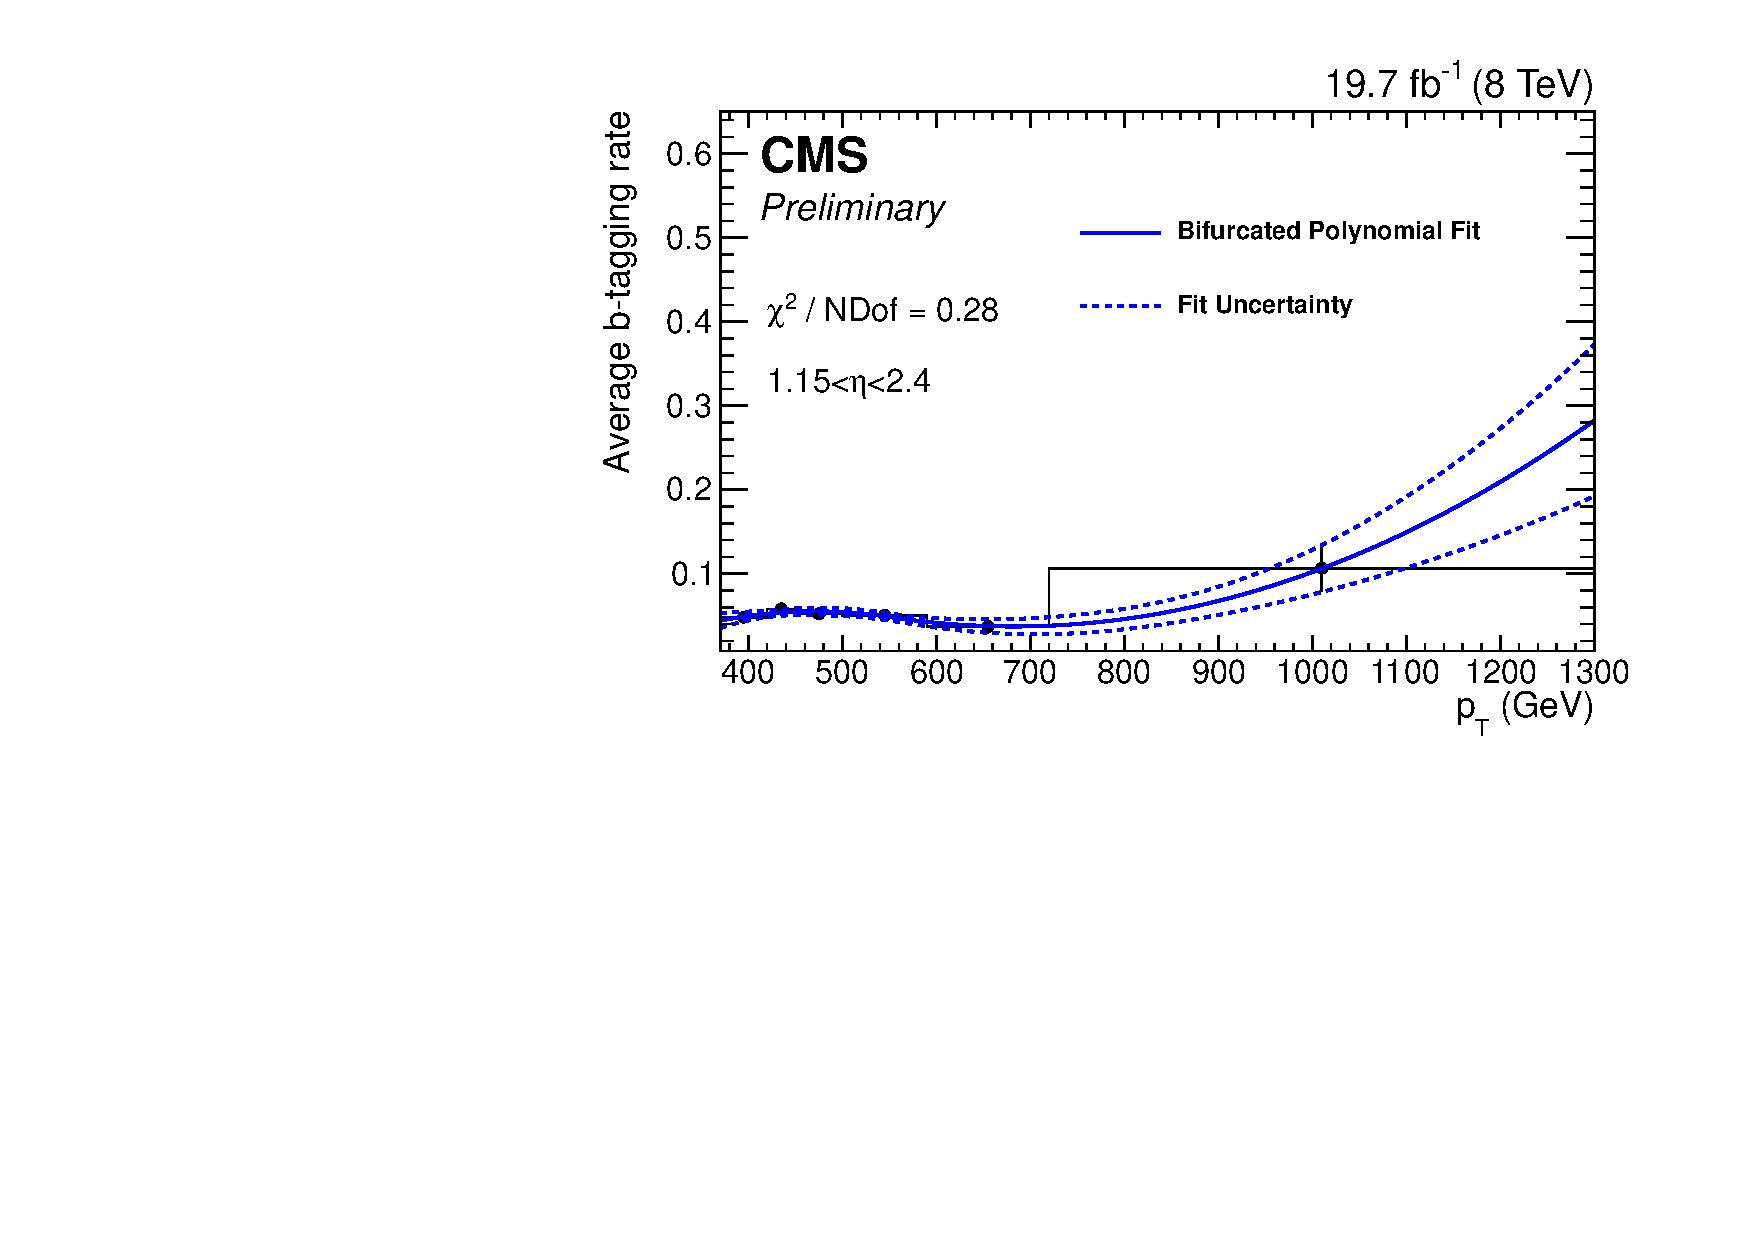
\includegraphics[width=0.7\textwidth]{AN-13-004/figs/tagrateeta3fitBP.pdf}}
\caption{
$\pt$ parameterized average b-tagging rate from
(a) Low $\eta$ region  
(b) Transition $\eta$ region 
(c) High $\eta$ region. 
  The average b-tagging rate is shown in black, the polynomial fit is shown in blue, and the propagated errors from the fit are shown as a blue dashed line.}
\label{figs:tagrateetafit}
\end{center}
\end{figure}

%\section{QCD Closure}
%As a closure test, the background estimation is performed on the QCD Monte Carlo samples listed in Table \ref{table:datasetsQCD}.  

%\begin{table}
%\begin{center}
%\begin{tabular}{|p{0.7\linewidth}|r|} 
%\hline
%\bf{Sample} & \bf{Cross-Section} \\
%\hline
%/QCD\_Pt-300to470\_TuneZ2star\_8TeV\_pythia6/Summer12-PU\_S7\_START52\_V9-v1/AODSIM & 1759.6 \\
%/QCD\_Pt-470to600\_TuneZ2star\_8TeV\_pythia6/Summer12-PU\_S7\_START52\_V9-v1/AODSIM & 113.9 \\
%/QCD\_Pt-600to800\_TuneZ2star\_8TeV\_pythia6/Summer12-PU\_S7\_START52\_V9-v1/AODSIM & 27.0 \\
%/QCD\_Pt-800to1000\_TuneZ2star\_8TeV\_pythia6/Summer12-PU\_S7\_START52\_V9-v1/AODSIM & 3.57 \\
%/QCD\_Pt-1000to1400\_TuneZ2star\_8TeV\_pythia6/Summer12-PU\_S7\_START52\_V9-v1/AODSIM & 0.738 \\
%/QCD\_Pt-1400to1800\_TuneZ2star\_8TeV\_pythia6/Summer12-PU\_S7\_START52\_V9-v1/AODSIM & 0.0335 \\
%\hline
%\end{tabular}
%\end{center}
%\caption{QCD Monte Carlo Sample.}
%\label{table:datasetsQCD}
%\end{table}

%The extracted tagrates are shown in Figure\ref{figs:tagrateetafitQCD}.  
%Here, the tagrate was extracted with the procedure noted in Sections \ref{sec:qcdBackgroundEstimationProcedure} 
%and \ref{sec:tagrateparameterization}, as the $\ttbar$ contribution is not present here.  The closure test was performed by using the tagrates to weigh 
%pre b tagged jets within the relevant $|\eta|$ and $\pt$ regions with the tagrate as fitted with the bifurcated polynomial fit outlined in Section \ref{sec:tagrateparameterization}.  For this closure test, 
%the tagrates were extracted from the sideband using only even numbered events from the Monte Carlo and applied to only the odd numbered events in the signal region.  
%The results are shown in Figure\ref{figs:QCDClosure}.    
%The Monte Carlo here is scaled to the total number of events in our full selection in data, and the error bars represent 
%$\sqrt{N}$ where N is the bin content.  This procedure allows us to investigate the effect of any possible bias given the current integrated luminosity.  The QCD closure analysis performed on the full statistic QCD sample can be seen in 
%\ref{figs:QCDClosure1}.  
%The tagrate comparison of signal region and sideband is shown in Figure\ref{figs:tagrateetaQCD_withSR}

%\begin{figure}[htcb]
%\begin{center}
%\subfigure{\label{figs:tagrateeta1fitBPQCD}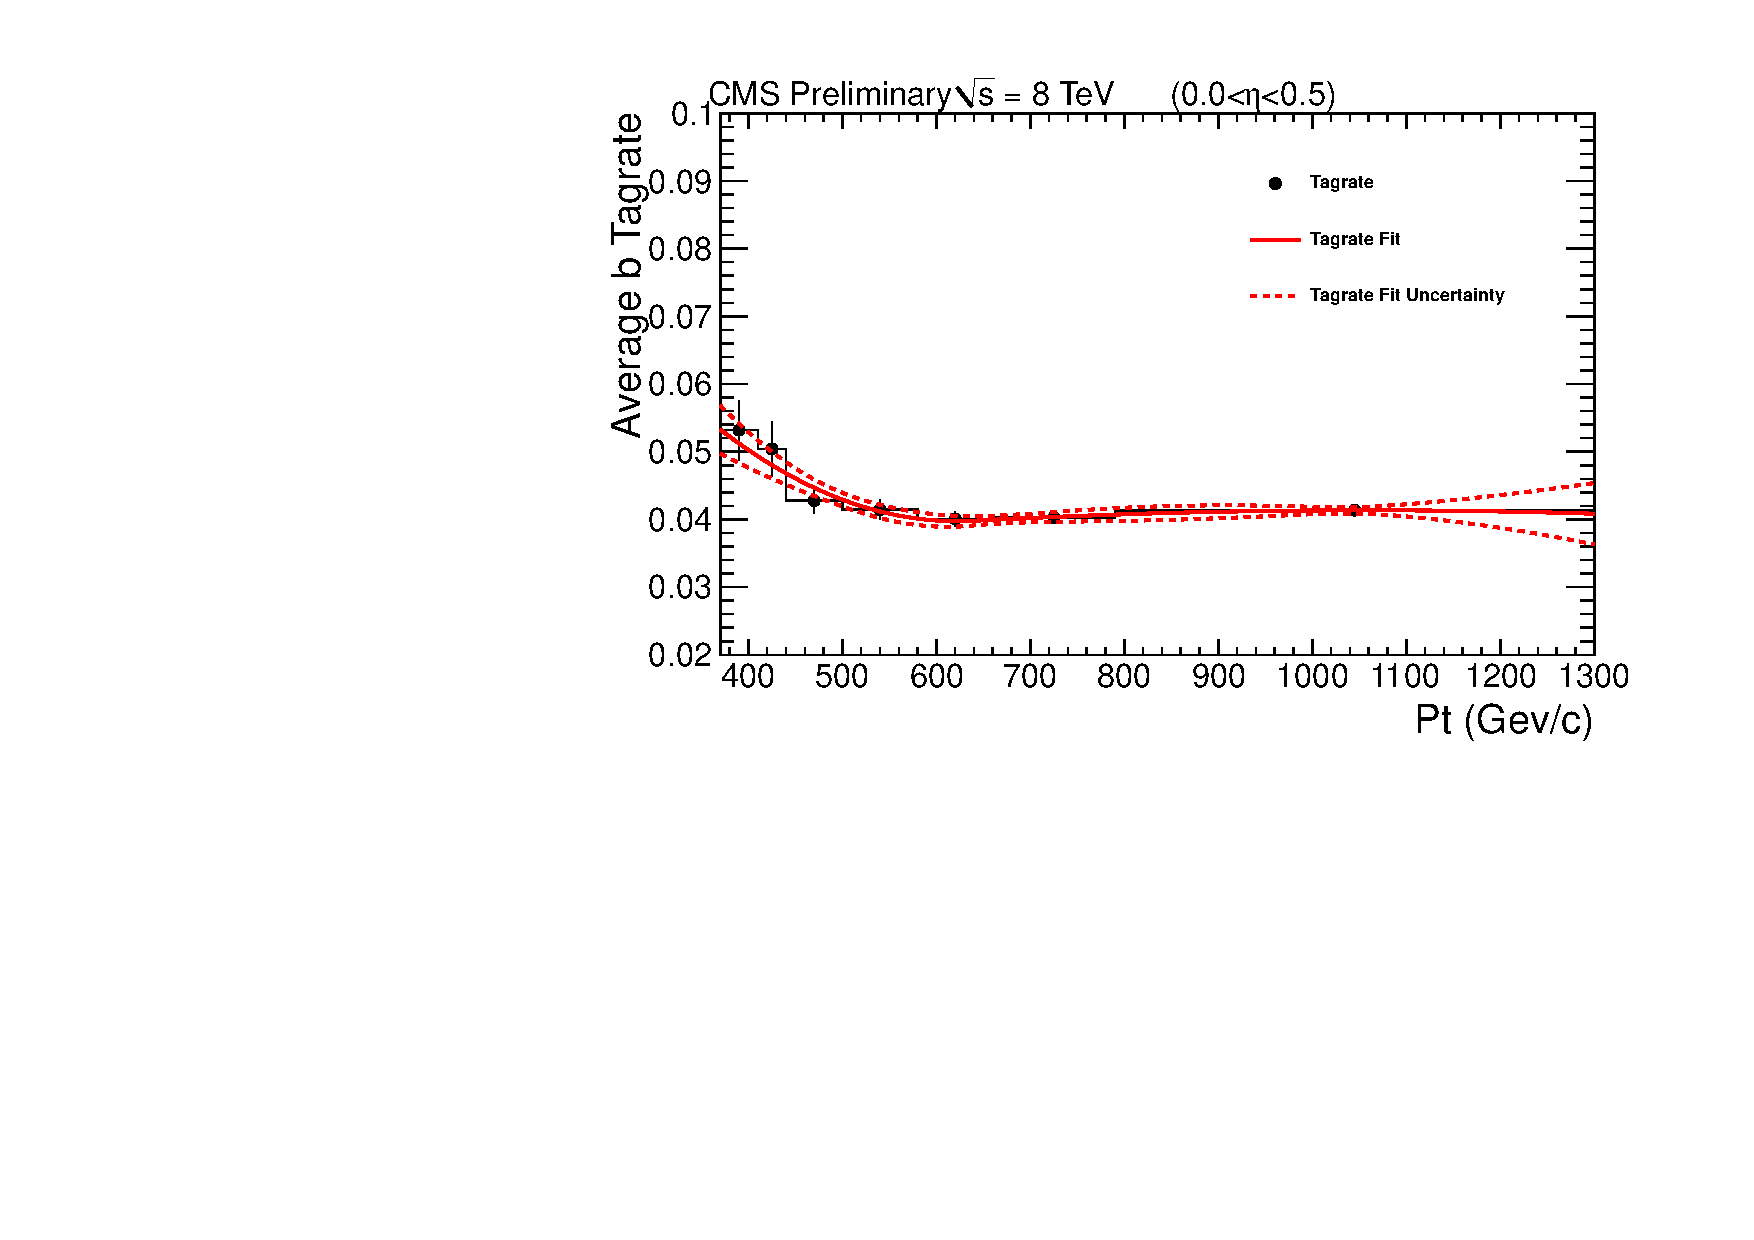
\includegraphics[width=0.75\textwidth]{AN-13-004/figs/tagrateeta1fitBPQCD.pdf}}\\
%\subfigure{\label{figs:tagrateeta2fitBPQCD}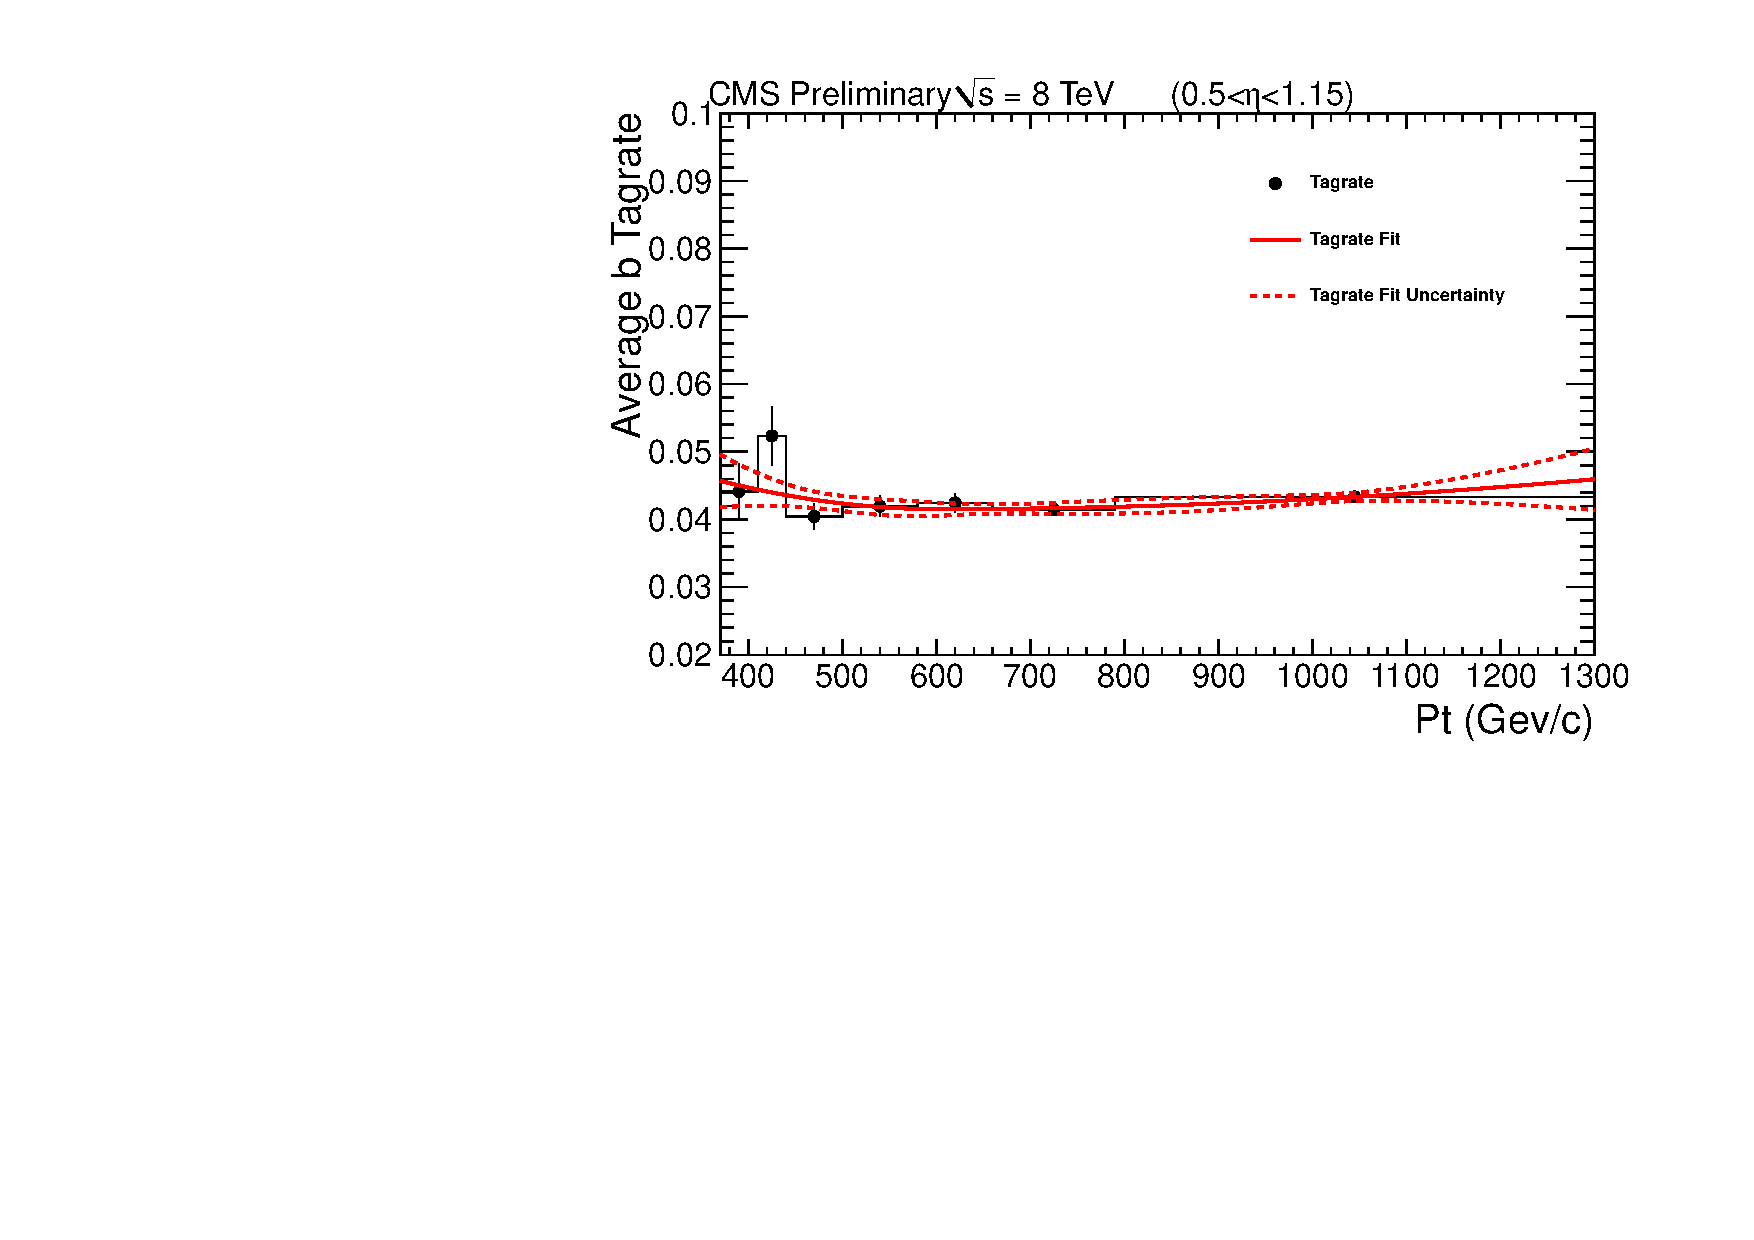
\includegraphics[width=0.75\textwidth]{AN-13-004/figs/tagrateeta2fitBPQCD.pdf}}\\
%\subfigure{\label{figs:tagrateeta3fitBPQCD}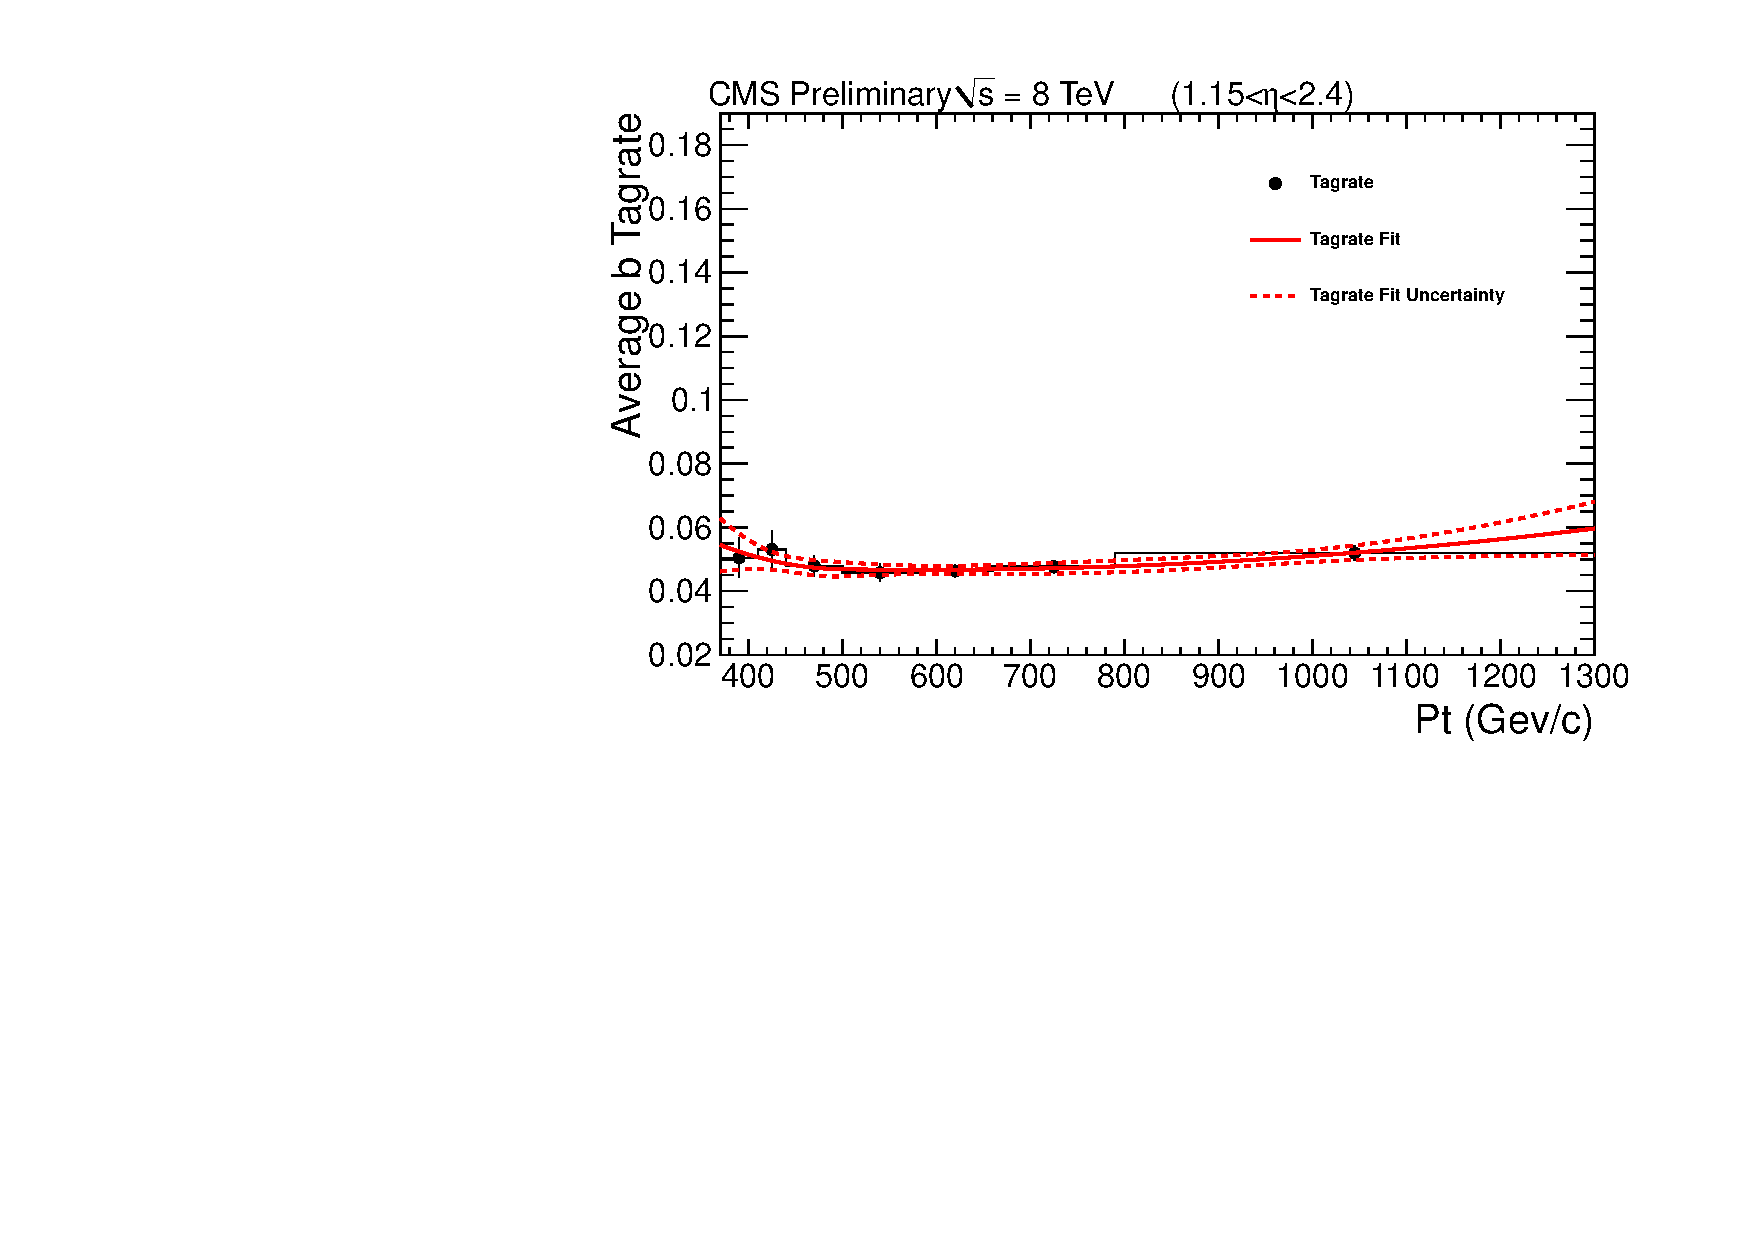
\includegraphics[width=0.75\textwidth]{AN-13-004/figs/tagrateeta3fitBPQCD.pdf}}
%\caption{
%QCD MC $\pt$ parameterized tagrate from
%(a) Low $\eta$ region  
%(b) Transition $\eta$ region 
%(c) High $\eta$ region 
%the average b-tagging rate is shown in black, the polynomial fit is shown in red, and the propagated errors from the fit are shown as a red dashed line.}
%\label{figs:tagrateetafitQCD}
%\end{center}
%\end{figure}

%\begin{figure}[htcb]
%\begin{center}
%\subfigure{\label{figs:tagrateeta1QCD_withSR}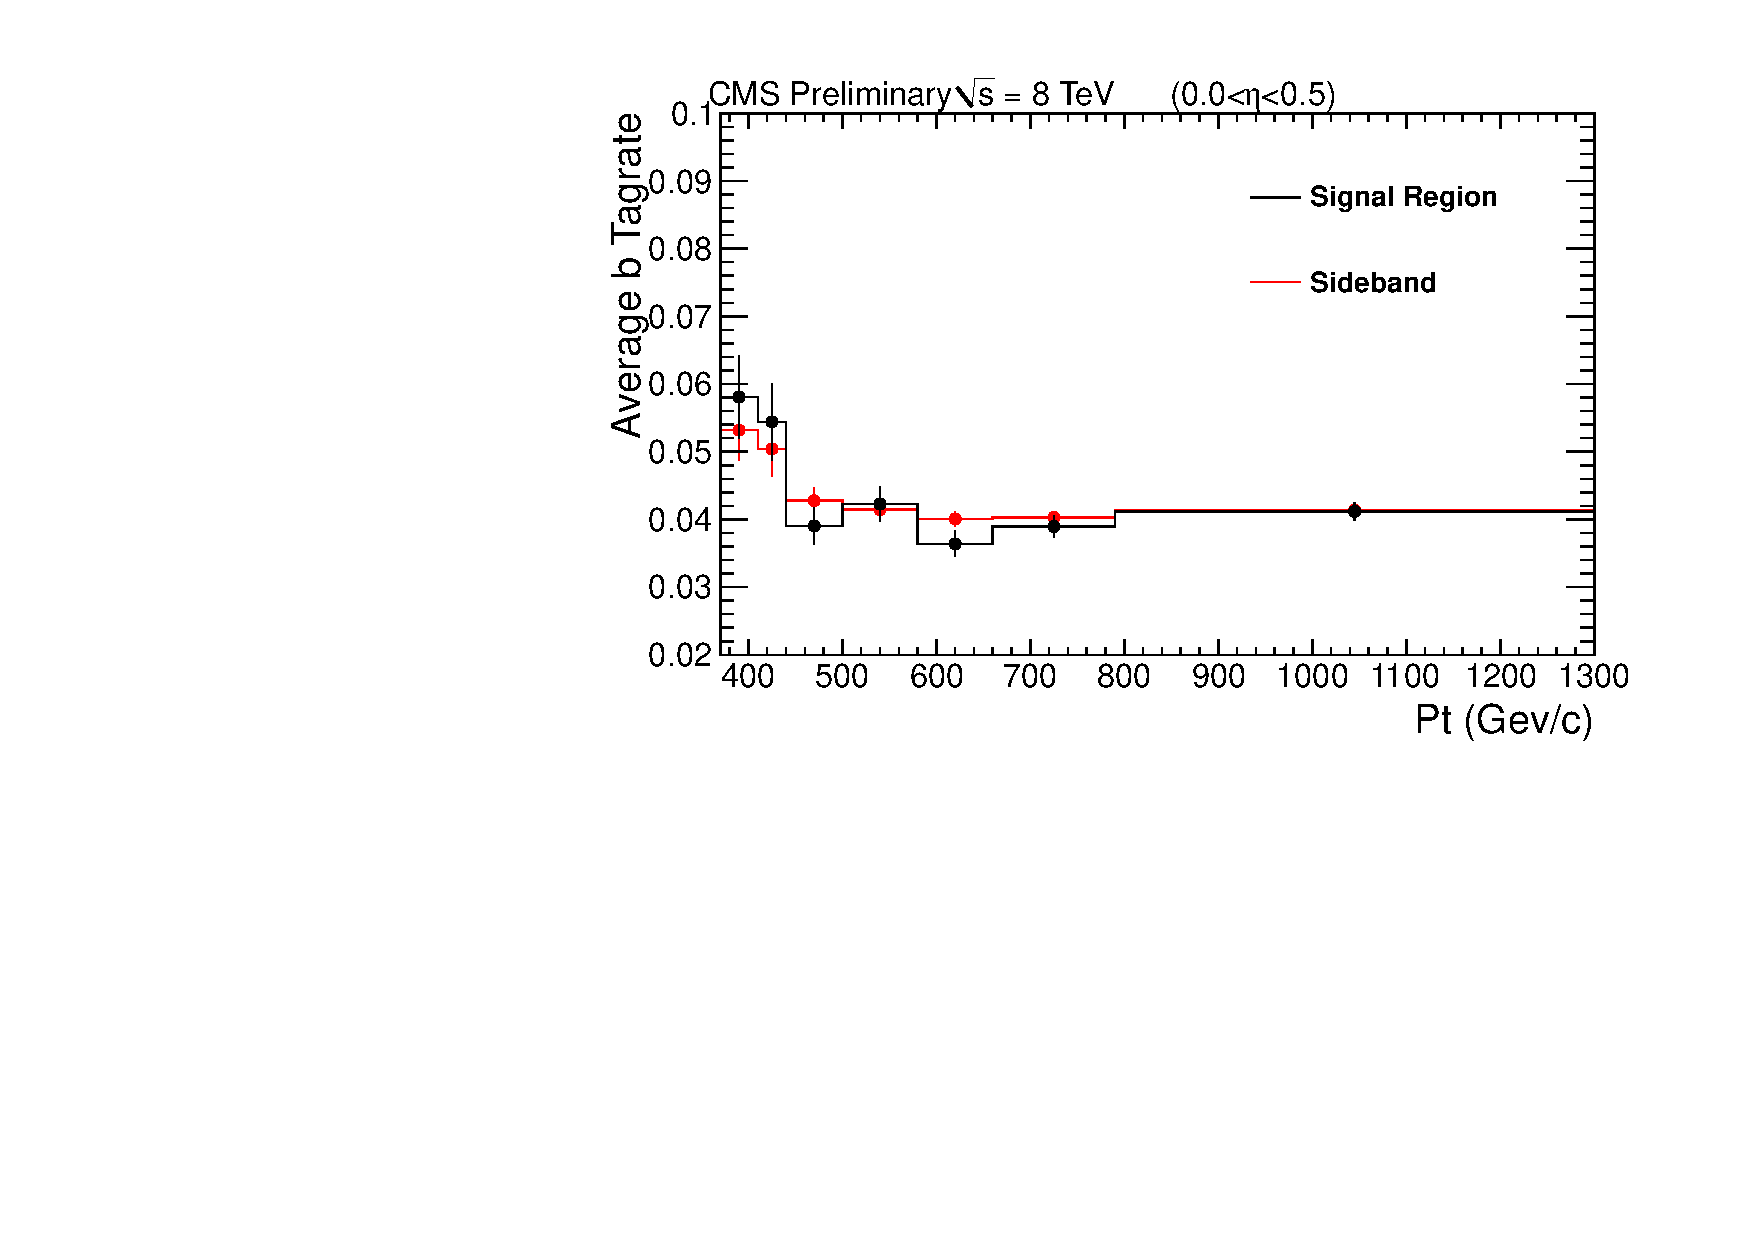
\includegraphics[width=0.75\textwidth]{AN-13-004/figs/tagrateeta1QCD_withSR}}\\
%\subfigure{\label{figs:tagrateeta2QCD_withSR}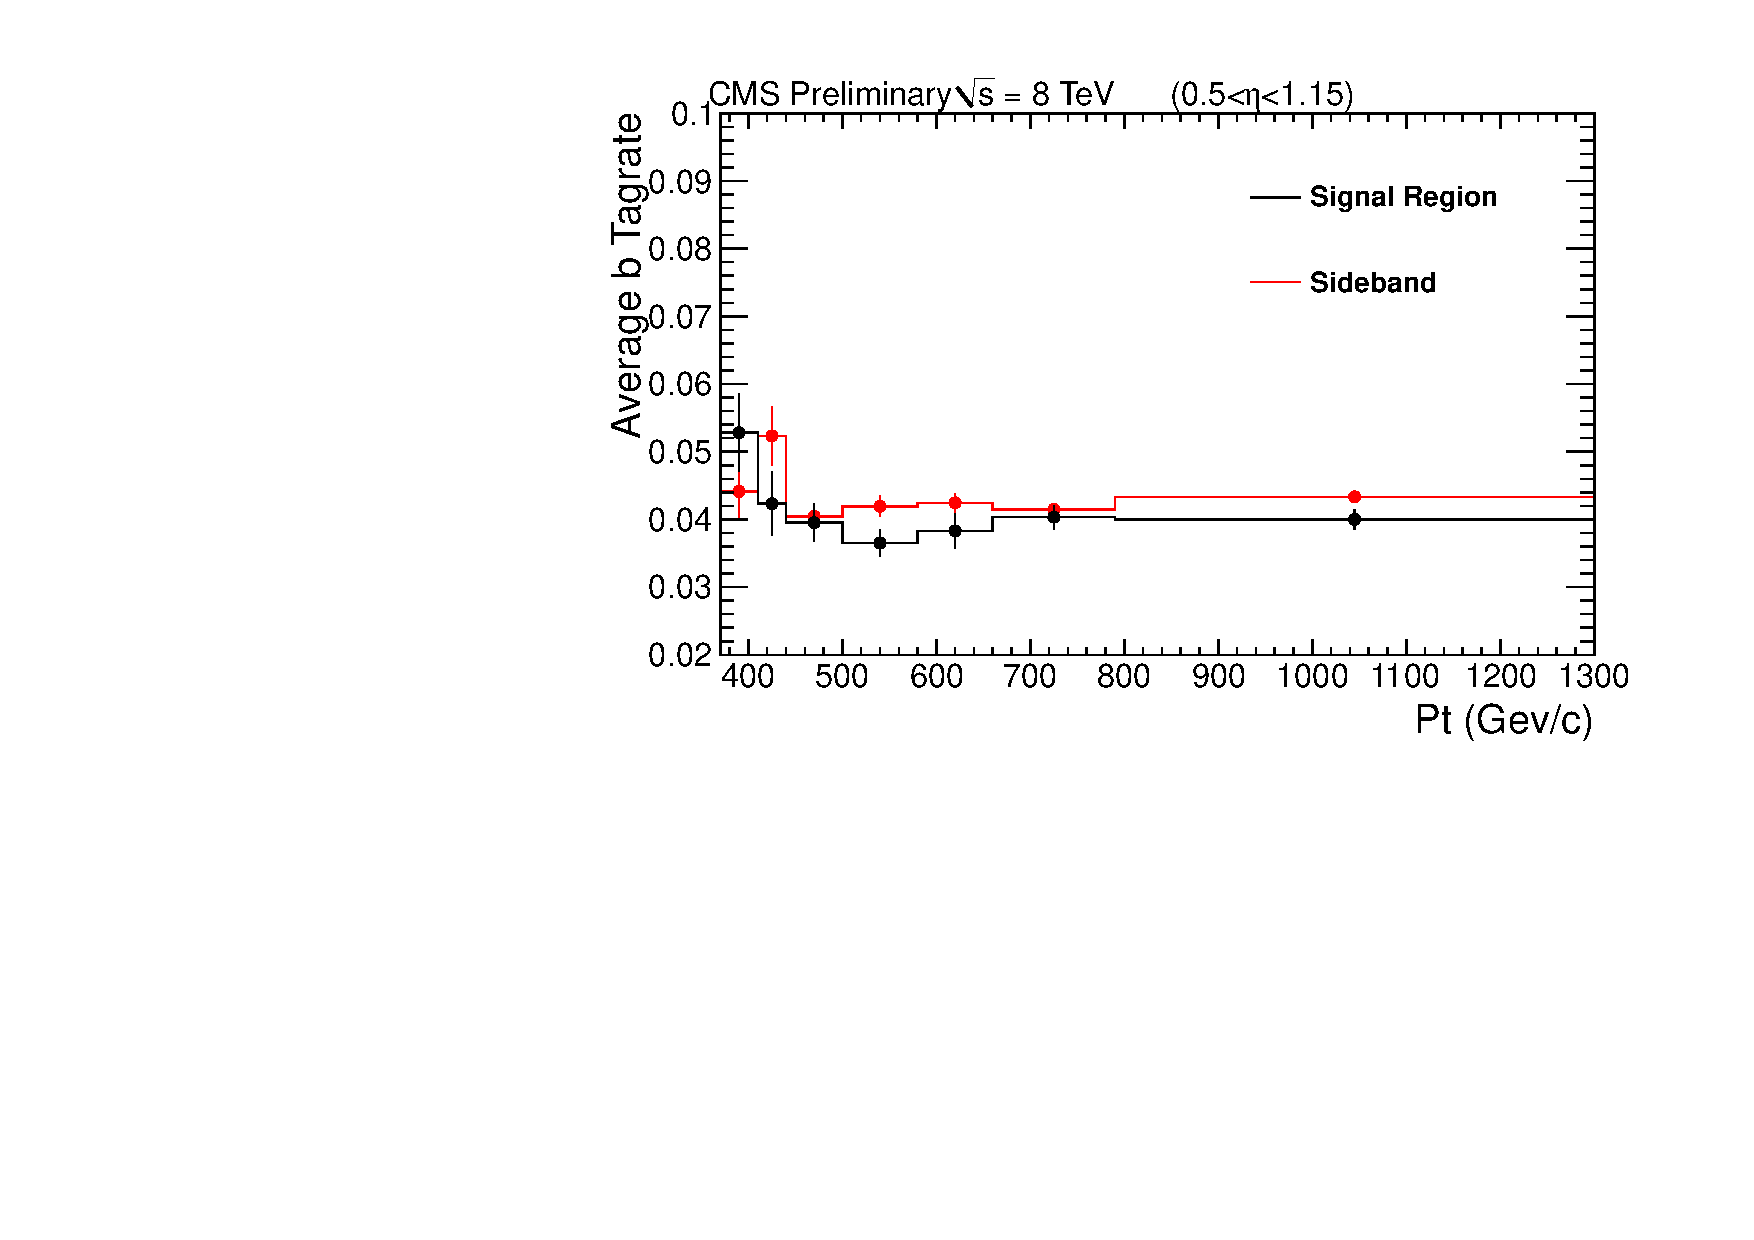
\includegraphics[width=0.75\textwidth]{AN-13-004/figs/tagrateeta2QCD_withSR}}\\
%\subfigure{\label{figs:tagrateeta3QCD_withSR}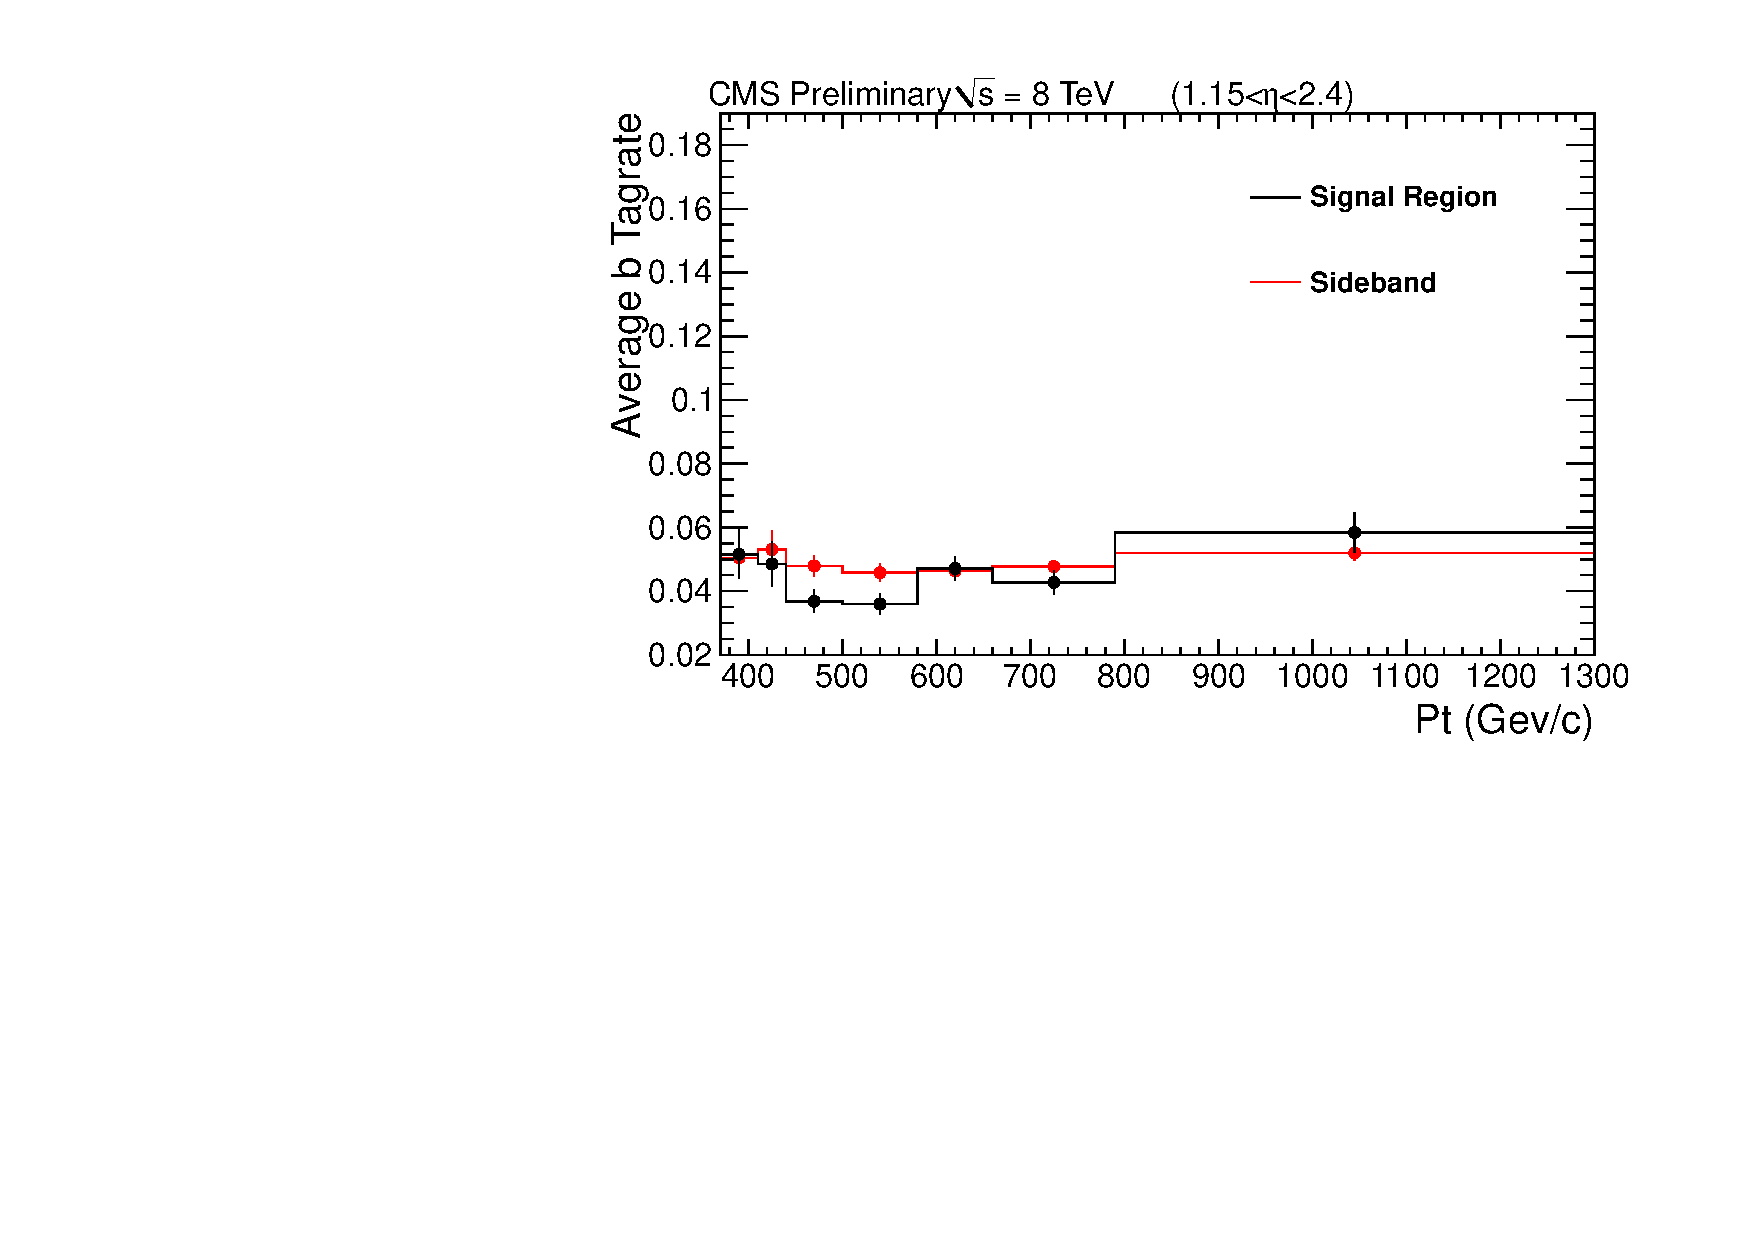
\includegraphics[width=0.75\textwidth]{AN-13-004/figs/tagrateeta3QCD_withSR}}
%\caption{
%QCD MC $\pt$ parameterized tagrate comparison to the signal region from
%(a) Low $\eta$ region  
%(b) Transition $\eta$ region 
%(c) High $\eta$ region 
%the average b-tagging rate from the Signal Region is shown in black, the average b-tagging rate from the Sideband is shown in red.}
%\label{figs:tagrateetaQCD_withSR}
%\end{center}
%\end{figure}

%\begin{figure}[htcb]
%\begin{center}
%\subfigure{\label{figs:MtbvsBkgQCDEO}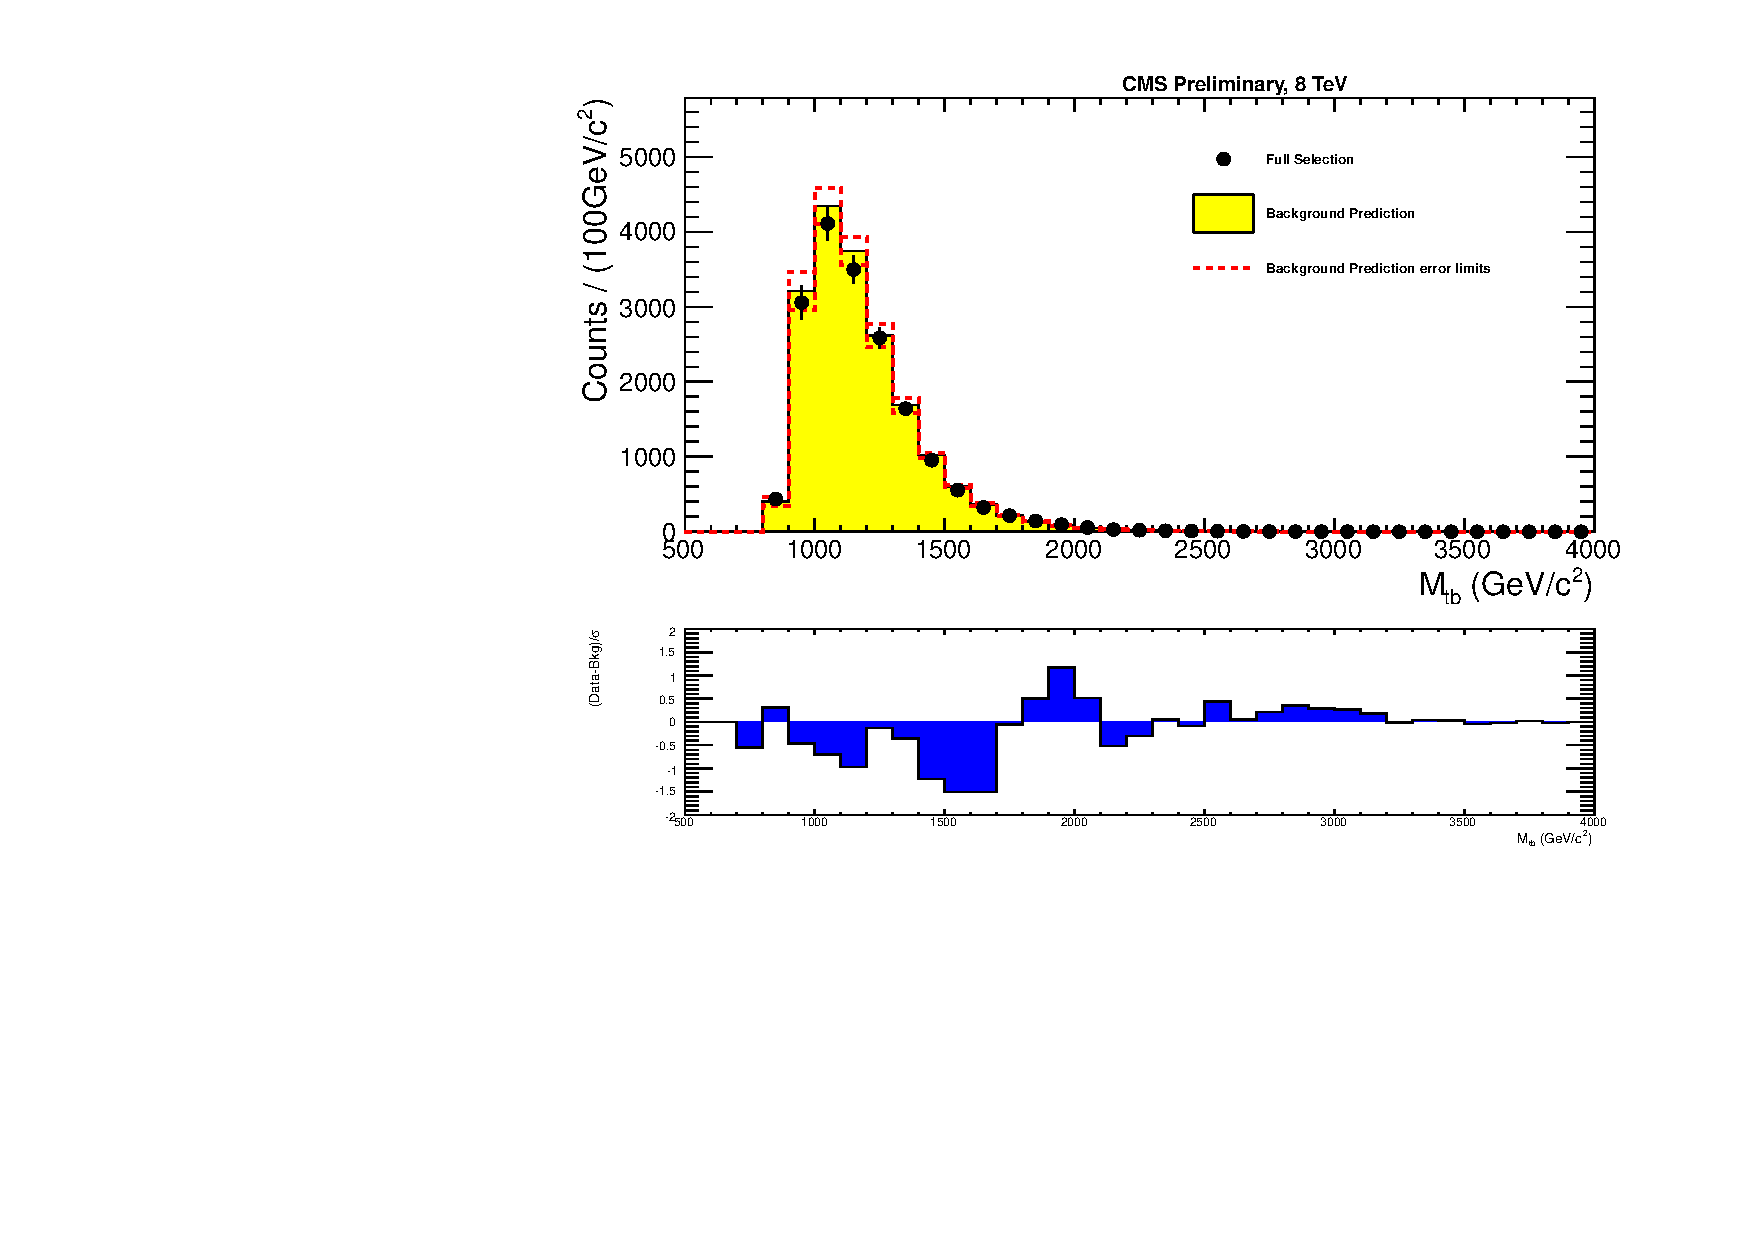
\includegraphics[width=1.0\textwidth]{AN-13-004/figs/MtbvsBkgQCDEO.pdf}}\\
%\subfigure{\label{figs:MtbvsBkgsemilog_QCDEO}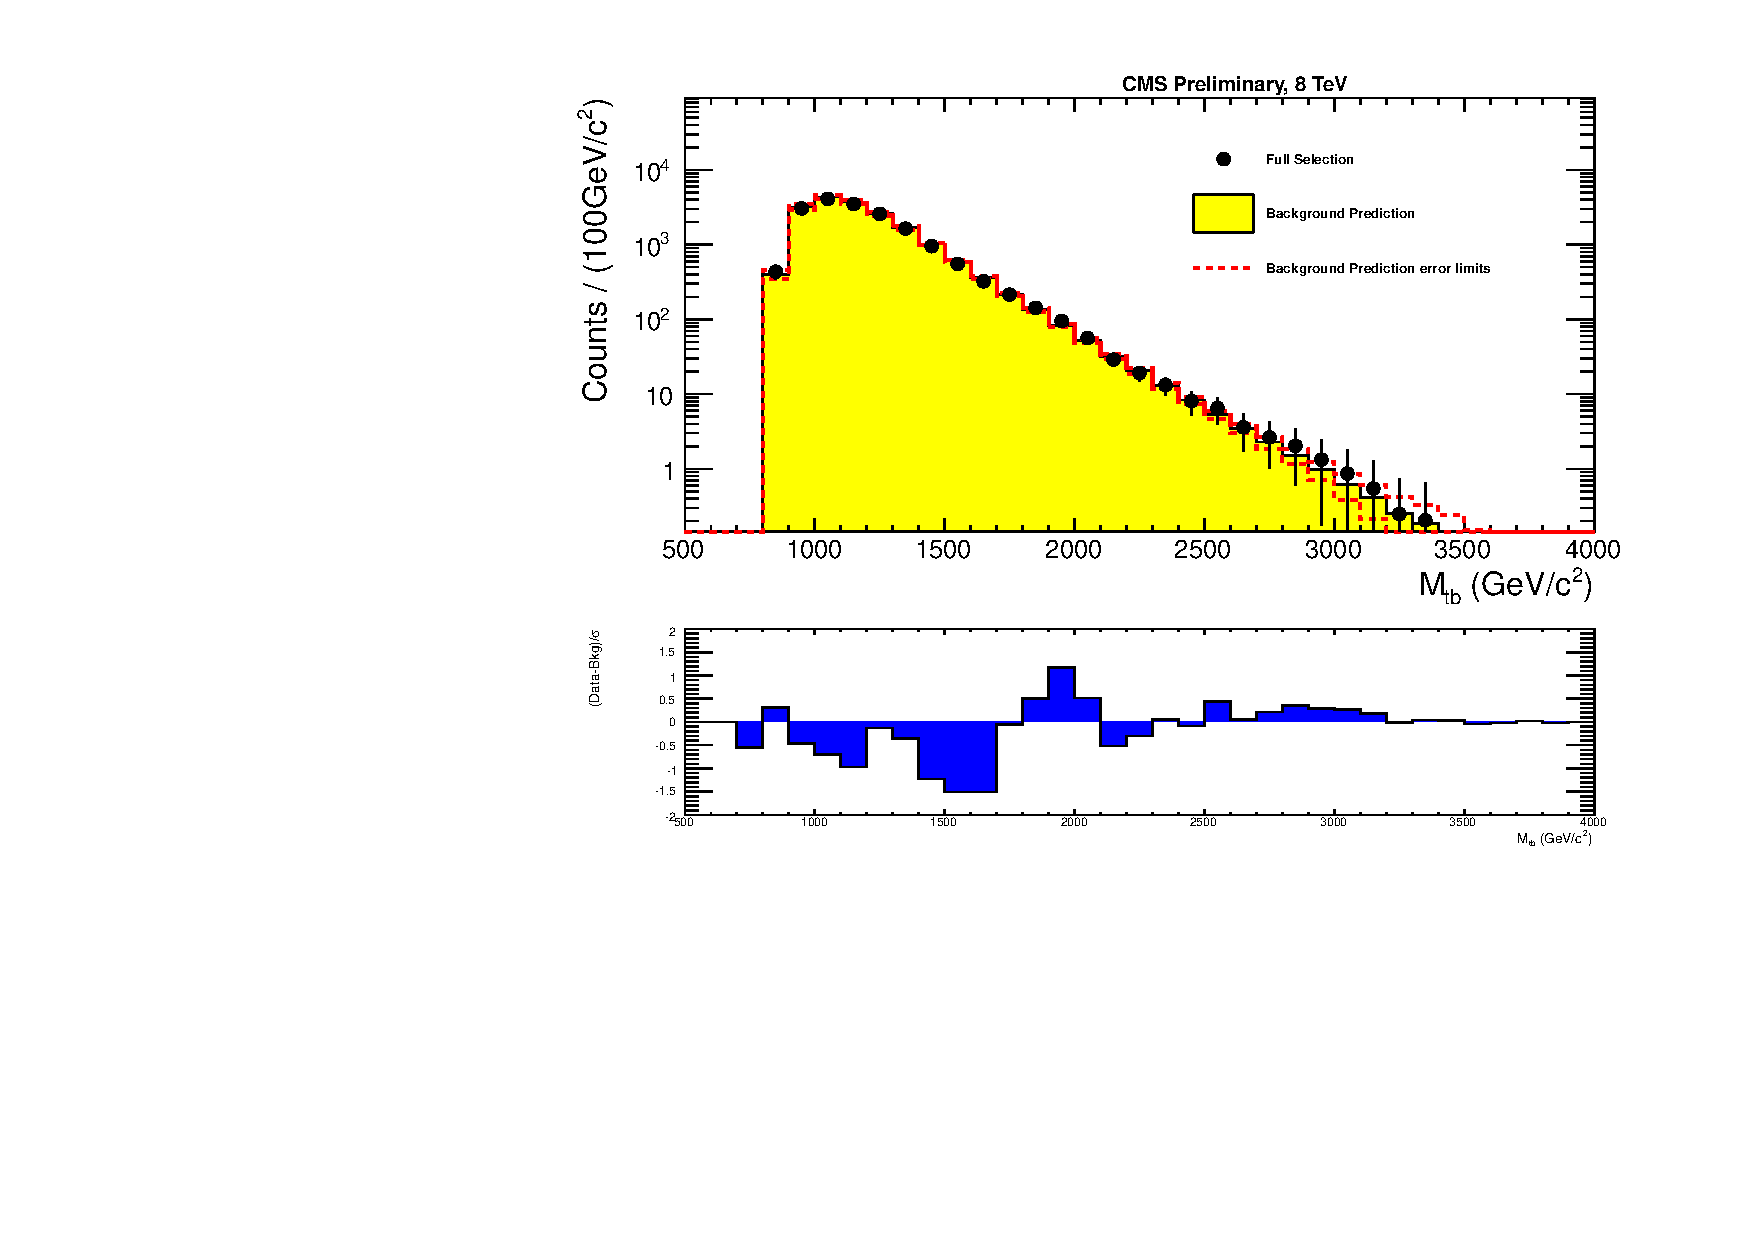
\includegraphics[width=1.0\textwidth]{AN-13-004/figs/MtbvsBkgsemilog_QCDEO.pdf}}
%\caption{
%QCD Monte Carlo background estimation closure test.  The background estimation is extracted from the tagrates shown in Figure\ref{figs:tagrateetafitQCD}.  The full selection is shown in black, 
%the background estimation is shown in yellow, and the errors from the background estimation are shown as a red dashed line.  Top and bottom plots are the same but on linear and log y-axis scale. }
%\label{figs:QCDClosure}
%\end{center}
%\end{figure}

\section{Sideband Closure}
\label{sec:secondsideband}
In order to investigate the applicability and versatility of the QCD background estimation in data, we apply the average b-tagging rate to sideband regions of our top tagging selection.  First, we define the following sideband:

\begin{itemize}
\item {\bf Jet Mass}  $\mathrm{\boldmath 140~\GeV < m_{\text{jet}} < 250~\GeV}$ 
\item {\bf Number of Subjets}  $\mathrm{\boldmath N_{\text{subjets}} > 2}$ 
\item {\bf Minimum Pairwise Mass} $\mathrm{\boldmath m_{\text{min}} \leq 50~\GeV}$ 
\item {\bf N-subjettiness} $\mathrm{\boldmath \tau_3/\tau_2 \geq 0.55}$ 
\item {\bf Subjet b-Tagging} $\mathrm{\boldmath SJ_{\text{CSVMAX}} \geq 0.679}$ 
\end{itemize}
This region lies outside of the signal region and sideband used for average b-tagging rate determination.  
The selection also has a very low yield of $\ttbar$, making it ideal for investigating the QCD background contribution.  
The average b-tagging rate used for this closure test is extracted from the same sideband as the signal region, and applied to pre-b-tagged events.  The closure test can be seen in Figure \ref{figs:NewMtbSB2}.

\begin{figure}[Htcb]
\centering
\subfigure{\label{figs:NewMtbSB21}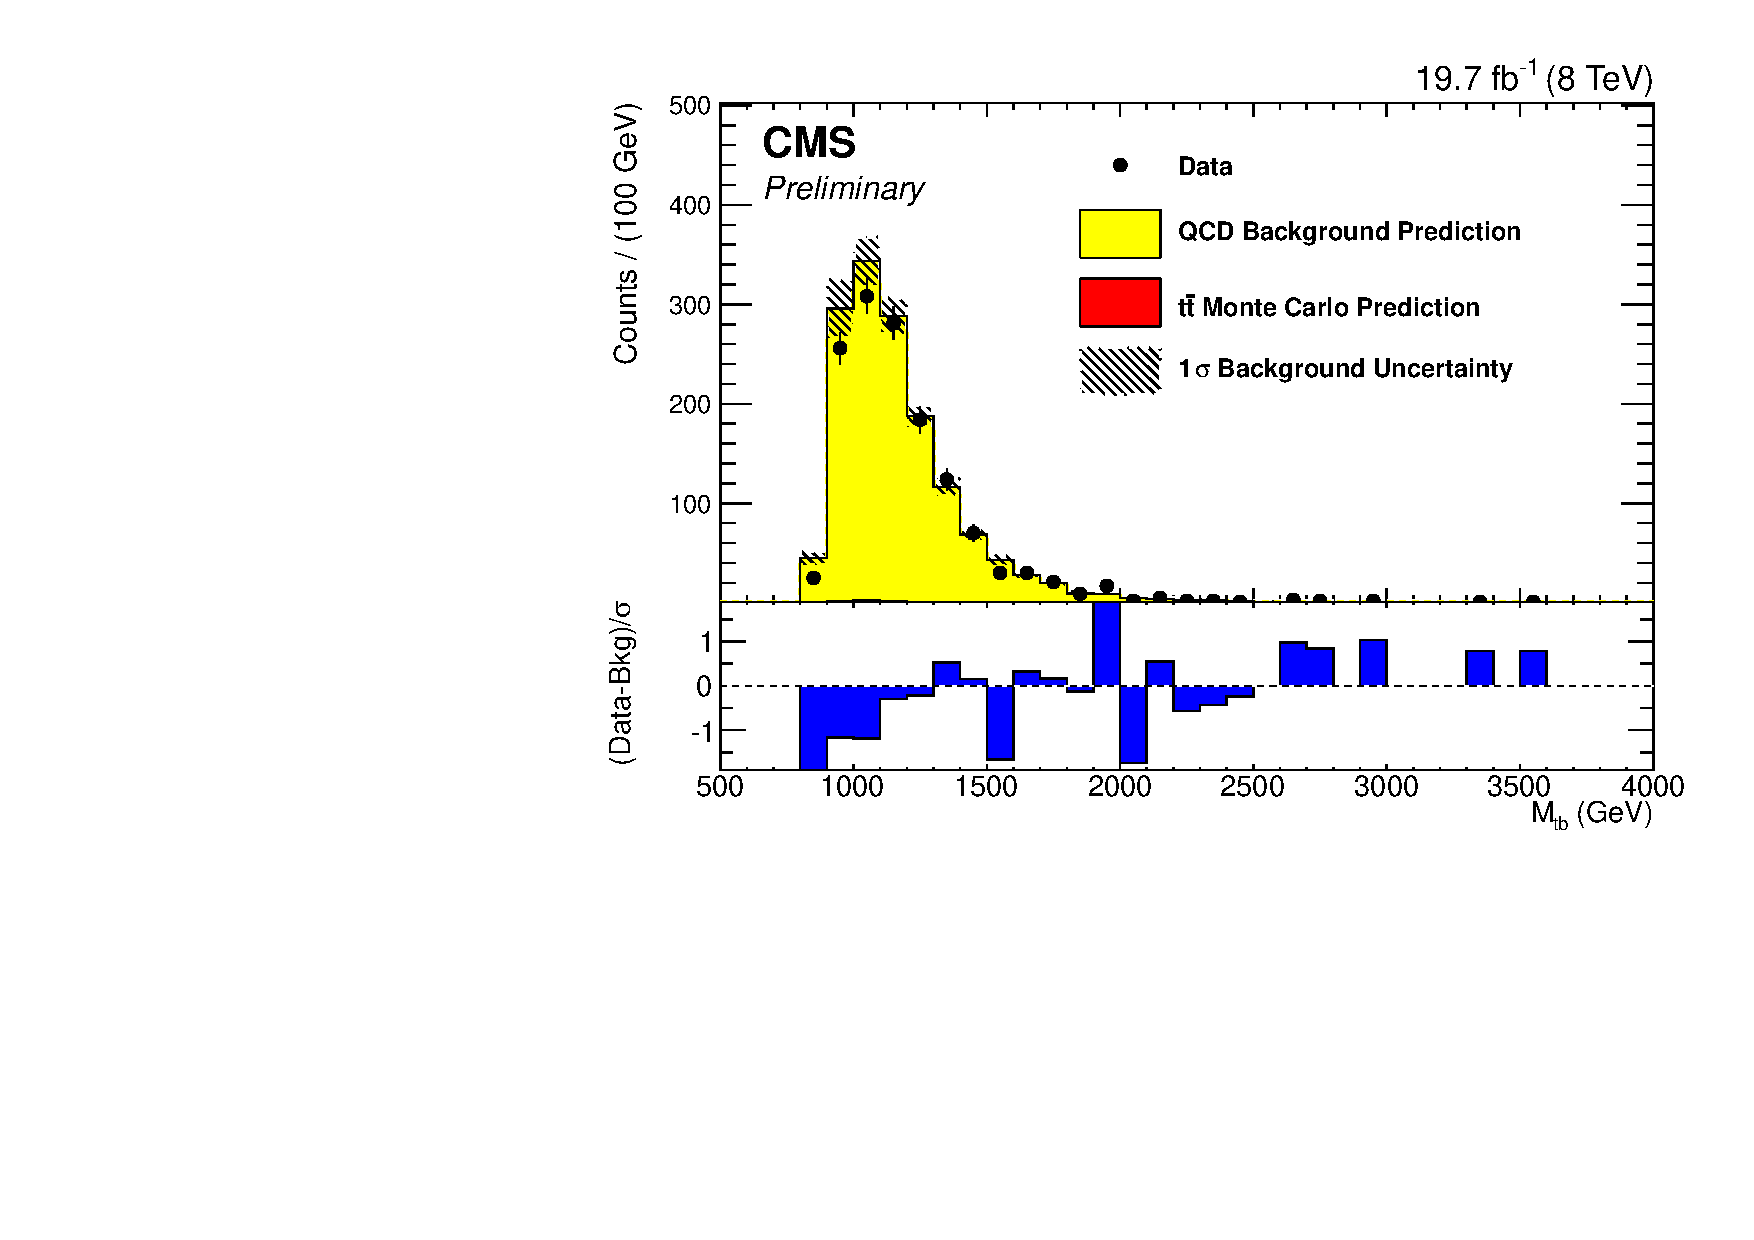
\includegraphics[width=.9\textwidth]{AN-13-004/figs/NewMtbSB2.pdf}}\\
\subfigure{\label{figs:NewMtbSB22}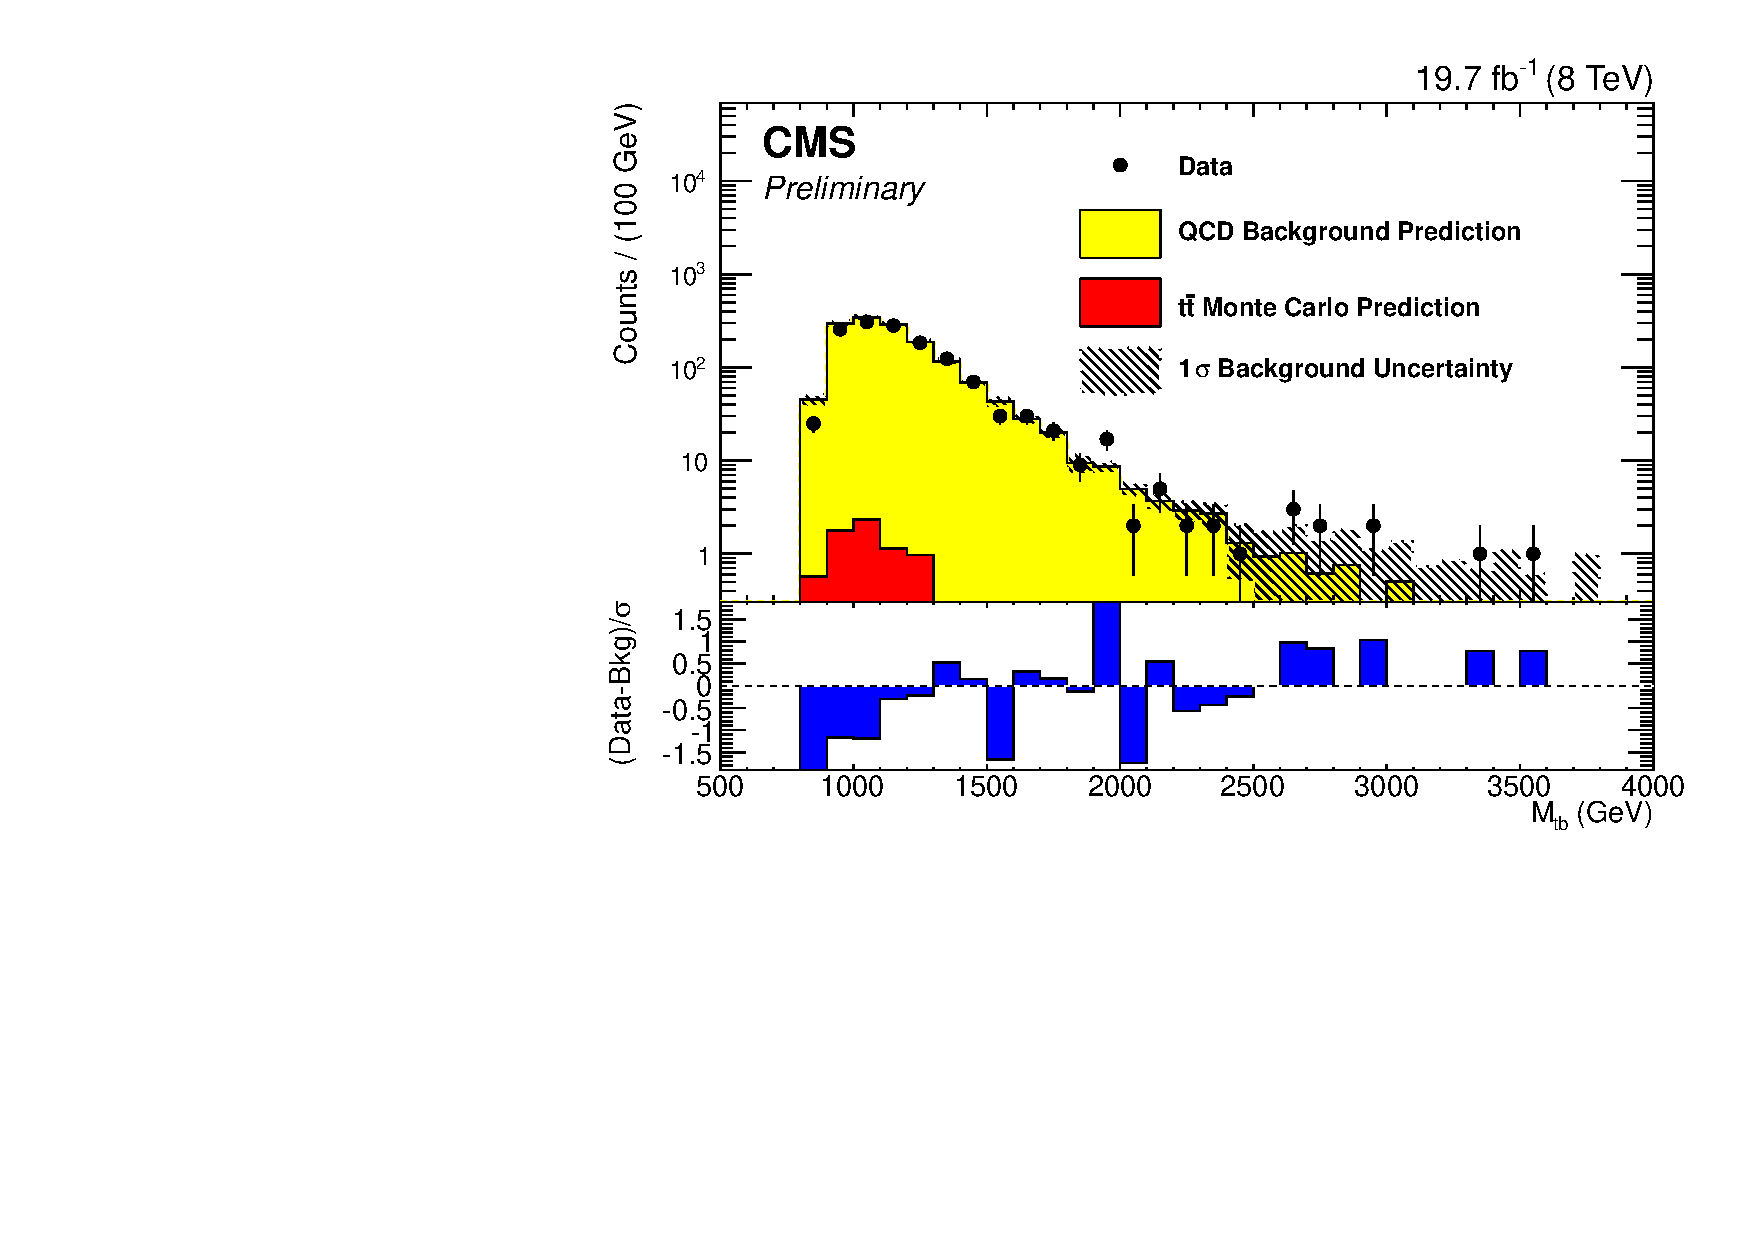
\includegraphics[width=.9\textwidth]{AN-13-004/figs/NewMtbSB2semilog.pdf}}
\caption{A plot of $M_{tb}$ in the control region defined by inverting the minimum pairwise mass and N-subjettiness cuts used in the full selection.  The top and bottom plots are the same but with linear and log y-axis scale.}
\label{figs:NewMtbSB2}
\end{figure}

Additionally, we can define the following sideband 
\begin{itemize}
\item {\bf Jet Mass}  $\mathrm{\boldmath 140~\GeV < m_{\text{jet}} < 250~\GeV}$ 
\item {\bf Number of Subjets}  $\mathrm{\boldmath N_{\text{subjets}} > 2}$ 
\item {\bf Minimum Pairwise Mass} $\mathrm{\boldmath m_{\text{min}} > 50~\GeV}$ 
\item {\bf N-subjettiness} $\mathrm{\boldmath \tau_3/\tau_2 < 0.55}$ 
\item {\bf Subjet b-Tagging} $\mathrm{\boldmath SJ_{\text{CSVMAX}} \leq 0.679}$ 
\end{itemize}
The closure test can be seen in Figure \ref{figs:NewMtbSB3}.

\begin{figure}[Htcb]
\centering
\subfigure{\label{figs:NewMtbSB31}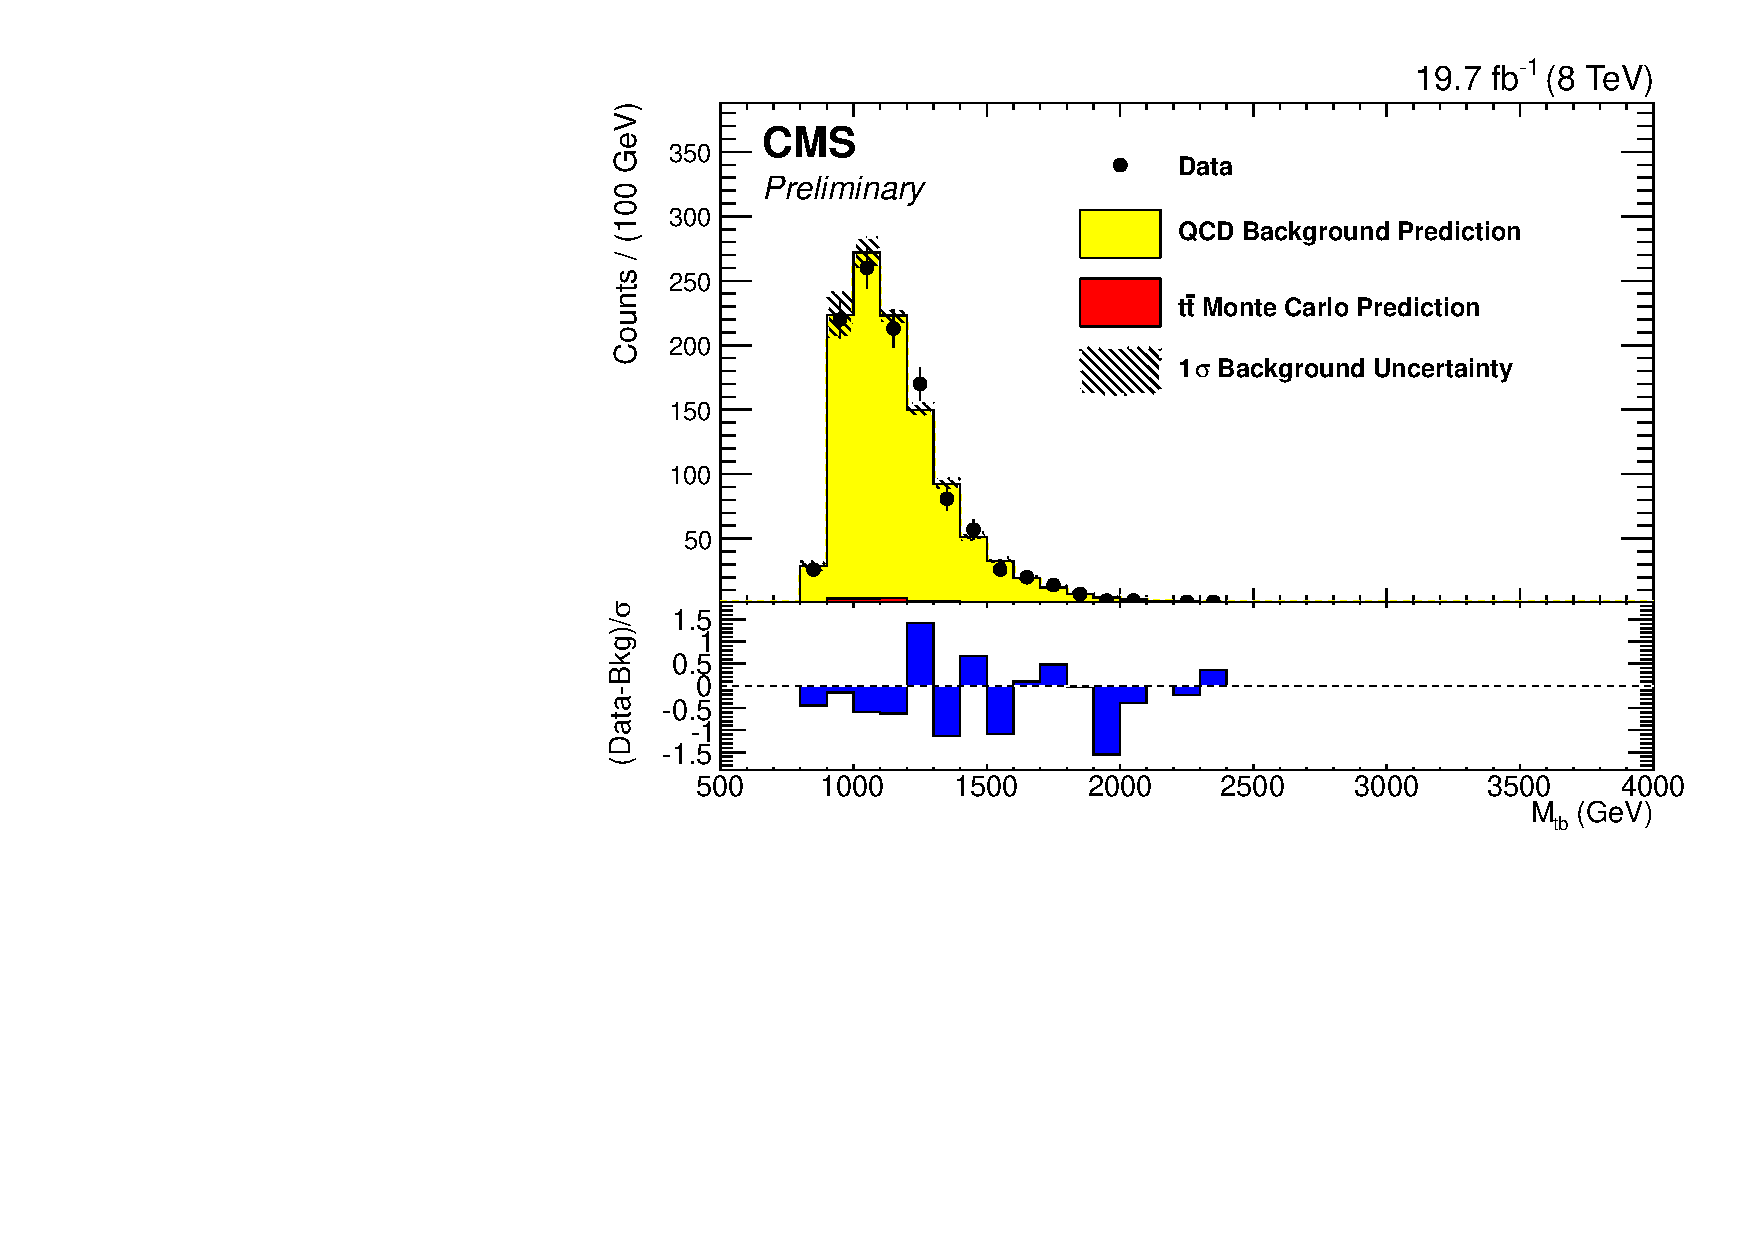
\includegraphics[width=.9\textwidth]{AN-13-004/figs/NewMtbSB3.pdf}}\\
\subfigure{\label{figs:NewMtbSB32}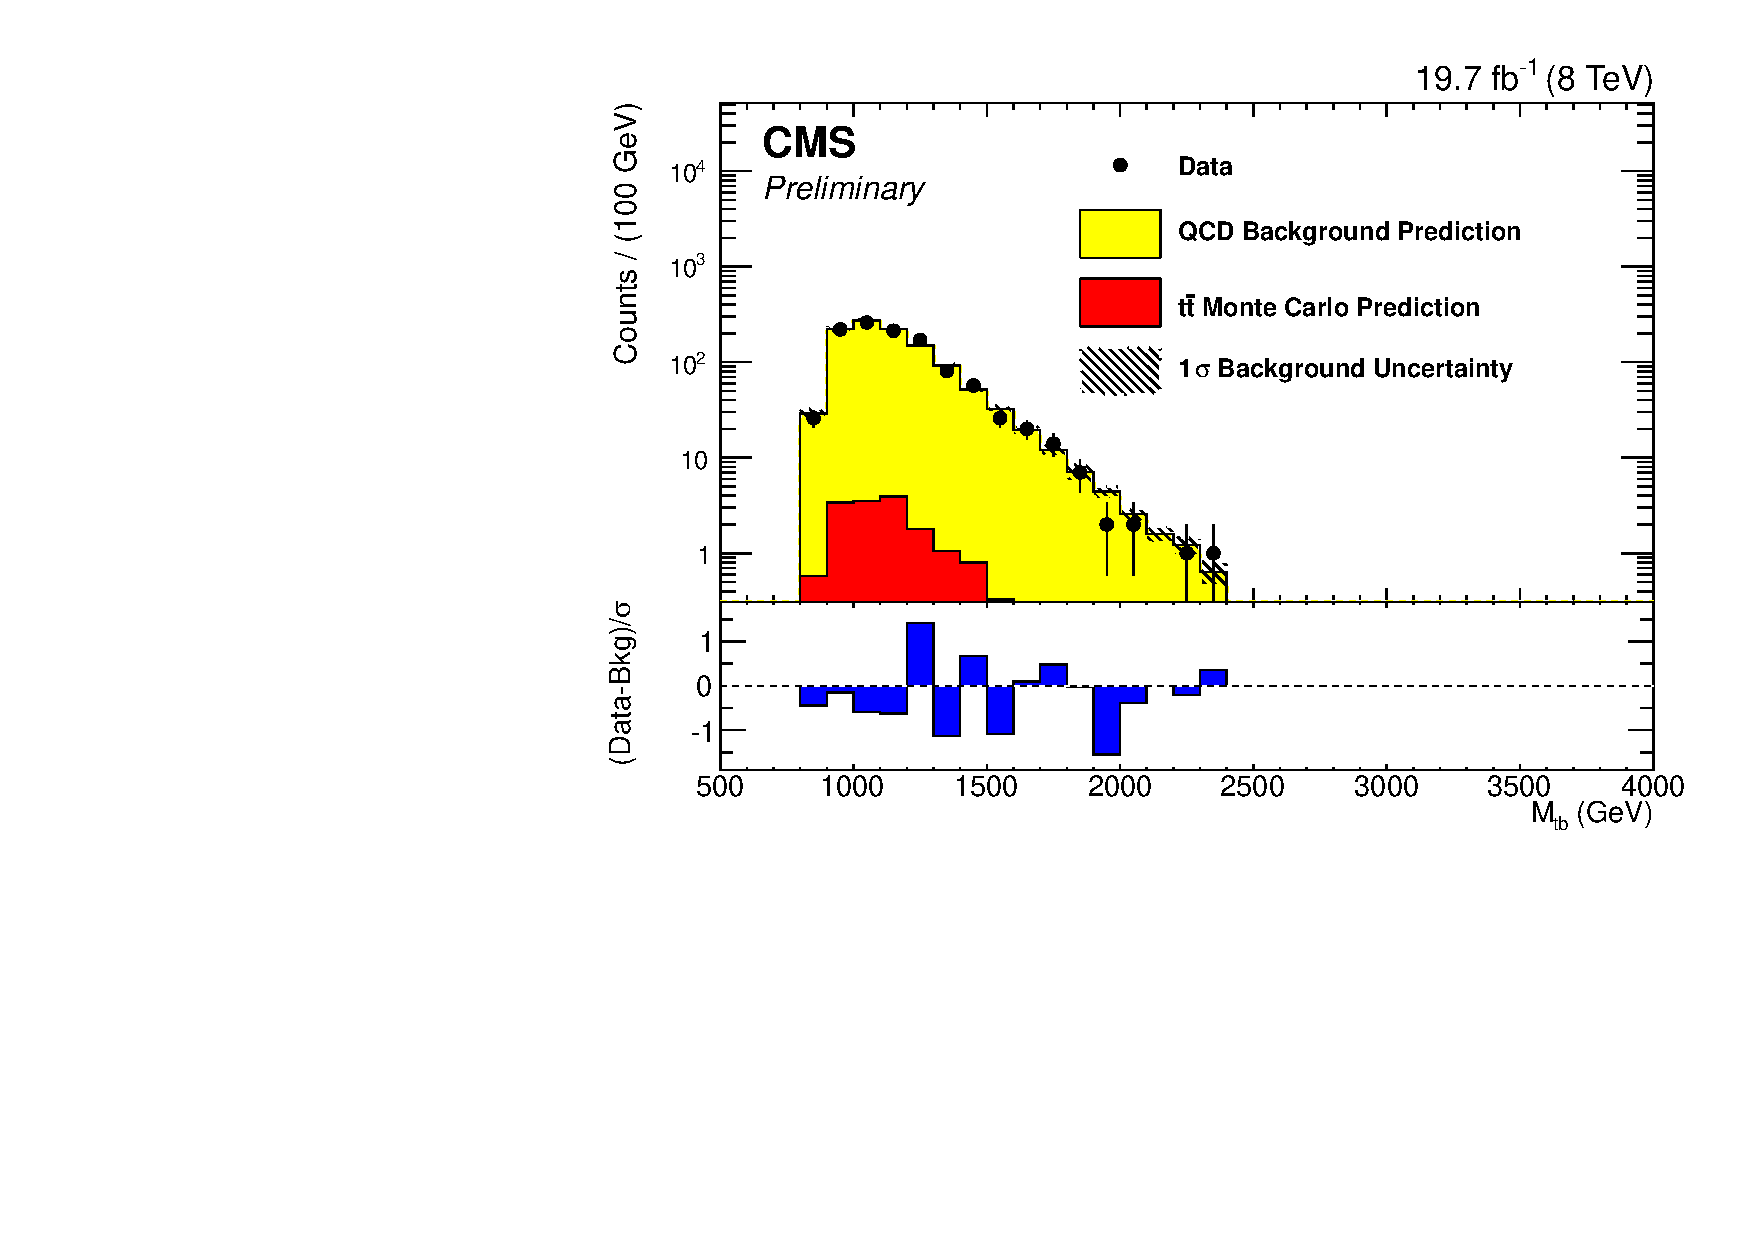
\includegraphics[width=.9\textwidth]{AN-13-004/figs/NewMtbSB3semilog.pdf}}
\caption{A plot of $M_{tb}$ in the control region defined by inverting the subjet b tagging cut used in the full selection.  The top and bottom plots are the same but with linear and log y-axis scale.}
\label{figs:NewMtbSB3}
\end{figure}

\section{Deriving the normalization of the SM $\ttbar$ production}
\label{sec:ttbarsideband}
In order to study the contribution from $\ttbar$ to tbe full background estimate, we turn to a sideband defined by inverting the b candidate mass requirement in the signal region.
This selection has an amplified $\ttbar$ fraction and is statistically independent from all other sidebands in the analysis.  
This makes the selection ideal for extracting the $\ttbar$ fraction in data.  
In order to extract this fraction, we compare the data-driven QCD background and $\ttbar$ Monte Carlo expectation to the selection in data.  

We perform a template fit to the invariant mass of the b 
candidate, using scaled $\ttbar$ Monte Carlo as one template, and the QCD background prediction as the other.  The fit allows
the QCD background template to move only within its errors, whereas the normalization on $\ttbar$ is unconstrained. 
The optimal parameterization for this fit is in a variable that has distinctly different shapes in $\ttbar$ and QCD.  
We therefore use the b candidate mass, which minimizes the correlation between the QCD and $\ttbar$ templates within the fit. The fit can be seen in Figure \ref{figs:ttbarfit}.  For this maximum likelihood fit we use the Theta package.

Additionally, the fit implements the $\ttbar$ subtraction in the QCD estimate by fitting un-subtracted QCD to the $\ttbar$ full selection.  The output of the fitter is then corrected by  
(1+S/F), where S/F is the ratio of the number of events in $\ttbar$ subtracted selection to the $\ttbar$ full selection. 

This study suggests after all scale factors applied in the analysis, the $\ttbar$ contribution needs to be amplified by $1.23 \pm 0.24$.  
This normalization is used for all $\ttbar$ distributions in the analysis, and the uncertainty is then the full normalization uncertainty for $\ttbar$.

\begin{figure}[htcb]
\centering
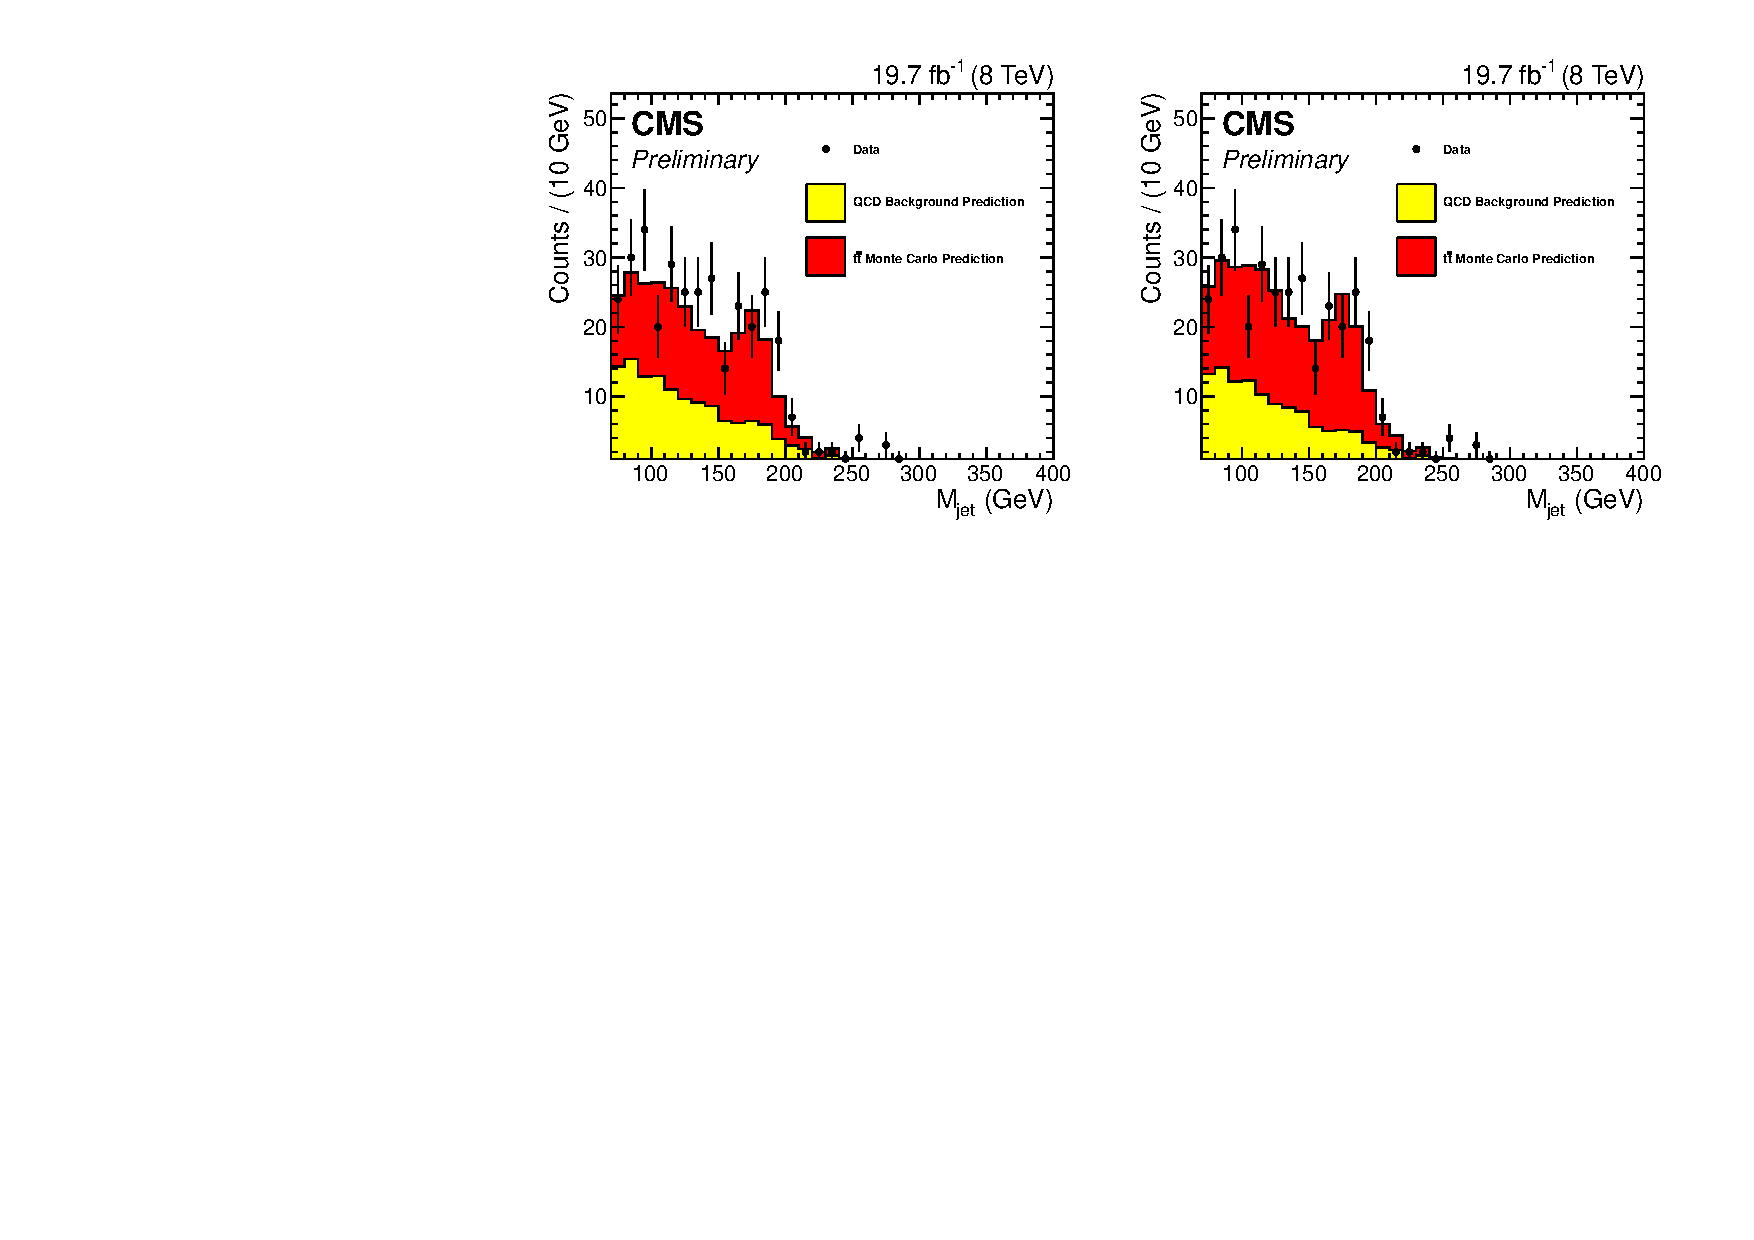
\includegraphics[width=1.0\textwidth]{AN-13-004/figs/ttbarfittingfromthetatmass}
\caption{b candidate mass as extracted from the b candidate mass inverted sideband.  Pre fraction fit (left) and post fraction fit (right).}
\label{figs:ttbarfit}
\end{figure}




